\documentclass[aspectratio=169,11pt]{beamer}

% Suppress default beamer navigation symbols
\setbeamertemplate{navigation symbols}{}

% Packages
\usepackage{fontspec}
\usepackage{graphicx}
\usepackage{tikz}
\usepackage{amsmath,amssymb}
\usepackage{ulem} % for \sout

% TikZ Libraries
\usetikzlibrary{arrows.meta,calc,positioning,shapes.geometric,backgrounds,fit,overlay-beamer-styles}

% ─────────────────────────────────────────────────────────────
% Color Palette: White Mode / Editorial Dossier Aesthetic
% ─────────────────────────────────────────────────────────────
\definecolor{boardbg}{HTML}{FFFFFF}
\definecolor{waveshape}{HTML}{E5DBC7}    % Warm kraft/sand organic wave matching slide theme
\definecolor{waveslate}{HTML}{1C2D3D}    % Deep rich slate wave backdrop
\definecolor{wavegold}{HTML}{C67D0A}     % Vibrant amber gold for 3D arrow     % Clean white presentation canvas
\definecolor{boardmid}{HTML}{F4F1EA}    % Subtle warm paper / panel tone
\definecolor{papercream}{HTML}{FAF7F0}  % Parchment card fill
\definecolor{paperdark}{HTML}{E5DEC9}   % Shaded card footer band
\definecolor{crimson}{HTML}{C1272D}     % Detective red string / alert
\definecolor{brass}{HTML}{8A5E1E}       % Antique brass / bronze header & labels
\definecolor{gold}{HTML}{B45309}        % Warm amber-gold highlight
\definecolor{chalk}{HTML}{181412}       % Deep typewriter charcoal ink (body & headers)
\definecolor{dimtext}{HTML}{6B5E4F}     % Muted annotation text
\definecolor{ink}{HTML}{14100E}         % Near-black typewriter ink
\definecolor{skyblue}{HTML}{1A6D88}     % Atmospheric slate-blue accent
\definecolor{biogreen}{HTML}{1B7436}    % Success / biology green

% Set beamer background
\setbeamercolor{background canvas}{bg=boardbg}

% ─────────────────────────────────────────────────────────────
% Typography (System Fonts)
% ─────────────────────────────────────────────────────────────
\setsansfont{Segoe UI}
\setmonofont{Courier New}
\newfontfamily\dispfont{Impact}
\newfontfamily\twfont{Courier New}

% ─────────────────────────────────────────────────────────────
% TikZ Styles
% ─────────────────────────────────────────────────────────────
\tikzset{
  gedge/.style={draw=crimson, line width=1.4pt},
  gedgeDim/.style={draw=dimtext!40, line width=0.8pt},
  gedgeVisible/.style={draw=brass!55, line width=0.9pt},
  gedgeHot/.style={draw=gold, line width=2.4pt},
  gnode/.style={circle, draw=brass, fill=boardmid, line width=1.5pt, minimum size=20pt, align=center},
  gnodeFocus/.style={circle, draw=gold, fill=boardmid, line width=2.5pt, minimum size=24pt, align=center},
  gnodeDim/.style={circle, draw=dimtext!50, fill=boardmid!80, line width=1.2pt, minimum size=20pt, align=center},
  gnodeWash/.style={circle, draw=dimtext!40, fill=dimtext!15, line width=1.2pt, minimum size=20pt, align=center},
  chip/.style={draw=brass!60, fill=boardmid, text=chalk, rounded corners=2pt, inner xsep=8pt, inner ysep=4pt, font=\fontsize{7.5}{9}\selectfont\twfont, align=center},
  chipFocus/.style={draw=gold, fill=boardmid, text=gold, rounded corners=2pt, inner xsep=8pt, inner ysep=4pt, font=\fontsize{7.5}{9}\selectfont\twfont\bfseries, align=center},
  bankbadge/.style={draw=brass, fill=boardmid, text=brass, rounded corners=2pt, inner xsep=8pt, inner ysep=4pt, font=\fontsize{7.5}{9}\selectfont\twfont\bfseries, align=center},
  scambadge/.style={draw=crimson, fill=boardmid, text=crimson, rounded corners=2pt, inner xsep=8pt, inner ysep=4pt, font=\fontsize{7.5}{9}\selectfont\twfont\bfseries, align=center},
  acard/.style={fill=papercream, text=ink, rounded corners=3pt, inner xsep=8pt, inner ysep=5pt, font=\fontsize{7.5}{9}\selectfont\sffamily, align=center},
  acardFocus/.style={draw=gold, line width=1.6pt, fill=papercream, text=ink, rounded corners=3pt, inner xsep=10pt, inner ysep=6pt, font=\fontsize{8}{10}\selectfont\sffamily, align=center}
}

% Header kicker macro
\newcommand{\kicker}[1]{%
  \begin{tikzpicture}[remember picture,overlay]
    \node[anchor=north west, text=brass,
          font=\fontsize{7}{7}\selectfont\twfont\bfseries,
          inner sep=0] at (current page.north west)
          [xshift=0.65cm, yshift=-0.38cm] {#1};
  \end{tikzpicture}%
}

% ─────────────────────────────────────────────────────────────
% Progressive-reveal helpers
% ─────────────────────────────────────────────────────────────
% `visible on=<2->` / `alt=<2>{..}{..}` come from overlay-beamer-styles.
\tikzset{
  gstep/.style={draw=brass!55, fill=boardmid, text=dimtext, rounded corners=2pt,
               inner xsep=7pt, inner ysep=4pt, align=center,
               font=\fontsize{7.5}{9}\selectfont\twfont},
  gstepon/.style={draw=gold, fill=boardmid, text=gold, rounded corners=2pt,
               inner xsep=7pt, inner ysep=4pt, align=center,
               font=\fontsize{7.5}{9}\selectfont\twfont\bfseries},
  % Person cards for the worked numeric demo
  pcard/.style={draw=brass!50, fill=papercream, text=ink, rounded corners=3pt,
                inner xsep=6pt, inner ysep=4pt, align=center},
  pcardHot/.style={draw=gold, line width=1.8pt, fill=papercream, text=ink,
                rounded corners=3pt, inner xsep=6pt, inner ysep=4pt, align=center},
  pcardDim/.style={draw=dimtext!55, fill=papercream!72!boardbg, text=ink!60,
                rounded corners=3pt, inner xsep=6pt, inner ysep=4pt, align=center},
  % Worksheet panel on the right half of the demo slides
  sheet/.style={draw=brass!45, fill=boardmid, rounded corners=3pt, line width=0.8pt},
  sline/.style={anchor=north west, text=chalk!88, align=left,
                font=\fontsize{8}{11}\selectfont\twfont},
  slineDim/.style={anchor=north west, text=dimtext, align=left,
                font=\fontsize{7.5}{10.5}\selectfont\twfont},
  slineHot/.style={anchor=north west, text=gold, align=left,
                font=\fontsize{8.5}{11.5}\selectfont\twfont\bfseries},
  shead/.style={anchor=north west, text=brass, align=left,
                font=\fontsize{8}{10}\selectfont\twfont\bfseries}
}

% Two-slot feature card body: {NAME}{activity}{topic}{topic colour}
% Fixed-width boxes keep the two columns aligned without a tabular
% (tabulars misbehave inside beamer frame bodies in this toolchain).
\newcommand{\prowa}[2]{%
  \makebox[1.15cm][l]{\fontsize{5.6}{7}\selectfont\twfont #1}%
  \makebox[0.58cm][r]{\fontsize{7.5}{9}\selectfont\twfont\bfseries #2}}
\newcommand{\prowb}[3]{%
  \makebox[1.15cm][l]{\fontsize{5.6}{7}\selectfont\twfont #1}%
  \makebox[0.58cm][r]{\fontsize{7.5}{9}\selectfont\twfont\bfseries\color{#3}#2}}
\newcommand{\pbody}[4]{%
  \begin{minipage}{1.75cm}\centering
    {\fontsize{8.5}{10}\selectfont\sffamily\bfseries #1}\par\vspace{1.5pt}
    \prowa{ACTIVITY}{#2}\par\vspace{1pt}
    \prowb{TOPIC X}{#3}{#4}
  \end{minipage}}

% Bare two-number vector chip: {activity}{topic}
\newcommand{\vecchip}[2]{$[\,\text{#1},\ \text{#2}\,]$}
\begin{document}

% =============================================================
% ACT I: THE GAP
% =============================================================

% --- 1.1-1.2: Cold Open · One card, then the network around it ---
\begin{frame}[plain]
\kicker{SCENE 01 / 17 \quad COLD OPEN}
\begin{tikzpicture}[remember picture,overlay,shift={(current page.center)}]

  % 1. Fluid organic wave backdrop on left (Warm paper/sand theme tone, NO GRID)
  \begin{scope}
    \clip (-8.5, -4.6) rectangle (3.0, 4.6);
    \fill[waveshape, draw=brass!40, line width=1.0pt] (-8.5, -4.6) -- (-8.5, 1.5)
      .. controls (-6.8, 0.6) and (-4.8, 0.8) .. (-3.0, 1.7)
      .. controls (-1.6, 2.4) and (-0.2, 2.3) .. (1.0, 1.2)
      .. controls (1.9, 0.3) and (2.3, -1.8) .. (2.5, -4.6) -- cycle;
  \end{scope}

  % 2. Glossy 3D accent sphere in top-left (warm gold matching theme)
  \shade[ball color=gold!85] (-6.8, 2.4) circle (0.36cm);
  \fill[white, opacity=0.6] (-6.9, 2.52) circle (0.09cm);

  % 3. Main header question on clean white canvas top
  \node[anchor=south west, text=chalk, font=\fontsize{22}{26}\selectfont\sffamily\bfseries, align=left]
    at (-7.2, 2.85) {\only<1-2>{Can we trust this person?}\only<3->{Look at the connections.}};

  % 4. Tilted Glassmorphic Card (matching reference style in warm editorial theme)
  \begin{scope}[shift={(-3.3, -0.4)}, rotate=4]
    % Drop shadow
    \fill[black!12, rounded corners=12pt] (-3.15, -1.65) rectangle (3.15, 1.45);
    % Card body in parchment cream with crisp brass contour
    \fill[papercream, rounded corners=12pt, draw=brass!50, line width=1.2pt] (-3.1, -1.6) rectangle (3.1, 1.4);
    \fill[paperdark, rounded corners=12pt, opacity=0.45] (-3.1, -1.6) rectangle (3.1, -0.65);

    % Small dossier label
    \node[anchor=north west, text=brass!90!ink, font=\fontsize{7}{8}\selectfont\twfont\bfseries]
      at (-2.8, 1.22) {DOSSIER $\cdot$ PROFILE \#10};
    \node[anchor=north east, text=ink!55, font=\fontsize{6.5}{7.5}\selectfont\twfont]
      at (2.8, 1.22) {PARIS / MADRID};

    % Giant bold focal title (Overlay 1-2: KYLIAN MBAPPÉ -> Overlay 3+: DICTATOR)
    \node[anchor=north west, font=\dispfont\fontsize{26}{28}\selectfont\bfseries]
      at (-2.8, 0.95) {\only<1-2>{\textcolor{gold}{KYLIAN MBAPPÉ}}\only<3->{\textcolor{crimson}{DICTATOR}}};

    % Thin divider positioned cleanly BELOW the big title
    \draw[ink!20, line width=0.5pt] (-2.8, -0.08) -- (2.8, -0.08);

    % Profile summary cues
    \node[anchor=north west, text=ink!85, font=\fontsize{7.5}{9.5}\selectfont\twfont]
      at (-2.8, -0.22) {\only<1-2>{AGE: 25 \quad FORWARD \quad 250+ GOALS}\only<3->{SUPREME COMMAND \quad TOTAL CONTROL}};

    % High-contrast status pill
    \node[anchor=center, font=\fontsize{8}{10}\selectfont\twfont\bfseries, align=center]
      at (0.0, -1.15) {\only<1-2>{\textcolor{biogreen!85!ink}{\textbf{WORLD CUP CHAMPION $\cdot$ CLEAN RECORD}}}\only<3->{\textcolor{crimson}{\textbf{TOTALITARIAN REGIME CONTEXT}}}};
  \end{scope}

  % 5. 3D curved accent arrow pointing towards Mbappé on overlay 1-2
  \begin{scope}[visible on=<1-2>]
    \draw[-{Latex[length=8pt,width=5.5pt]}, black!15, line width=3.4pt, cap=round]
      (0.2, 1.2) to[bend left=28] (2.2, 1.5);
    \draw[-{Latex[length=8pt,width=5.5pt]}, gold, line width=3.2pt, cap=round]
      (0.2, 1.25) to[bend left=28] (2.2, 1.55);
    \draw[white!70, line width=1.0pt, cap=round]
      (0.4, 1.35) to[bend left=26] (1.9, 1.62);
  \end{scope}

  % 6. Right side: Mbappé Cutout (Shifted slightly right for optimal spacing)
  \node[anchor=south, inner sep=0pt, visible on=<1-2>] at (4.6, -4.5)
    {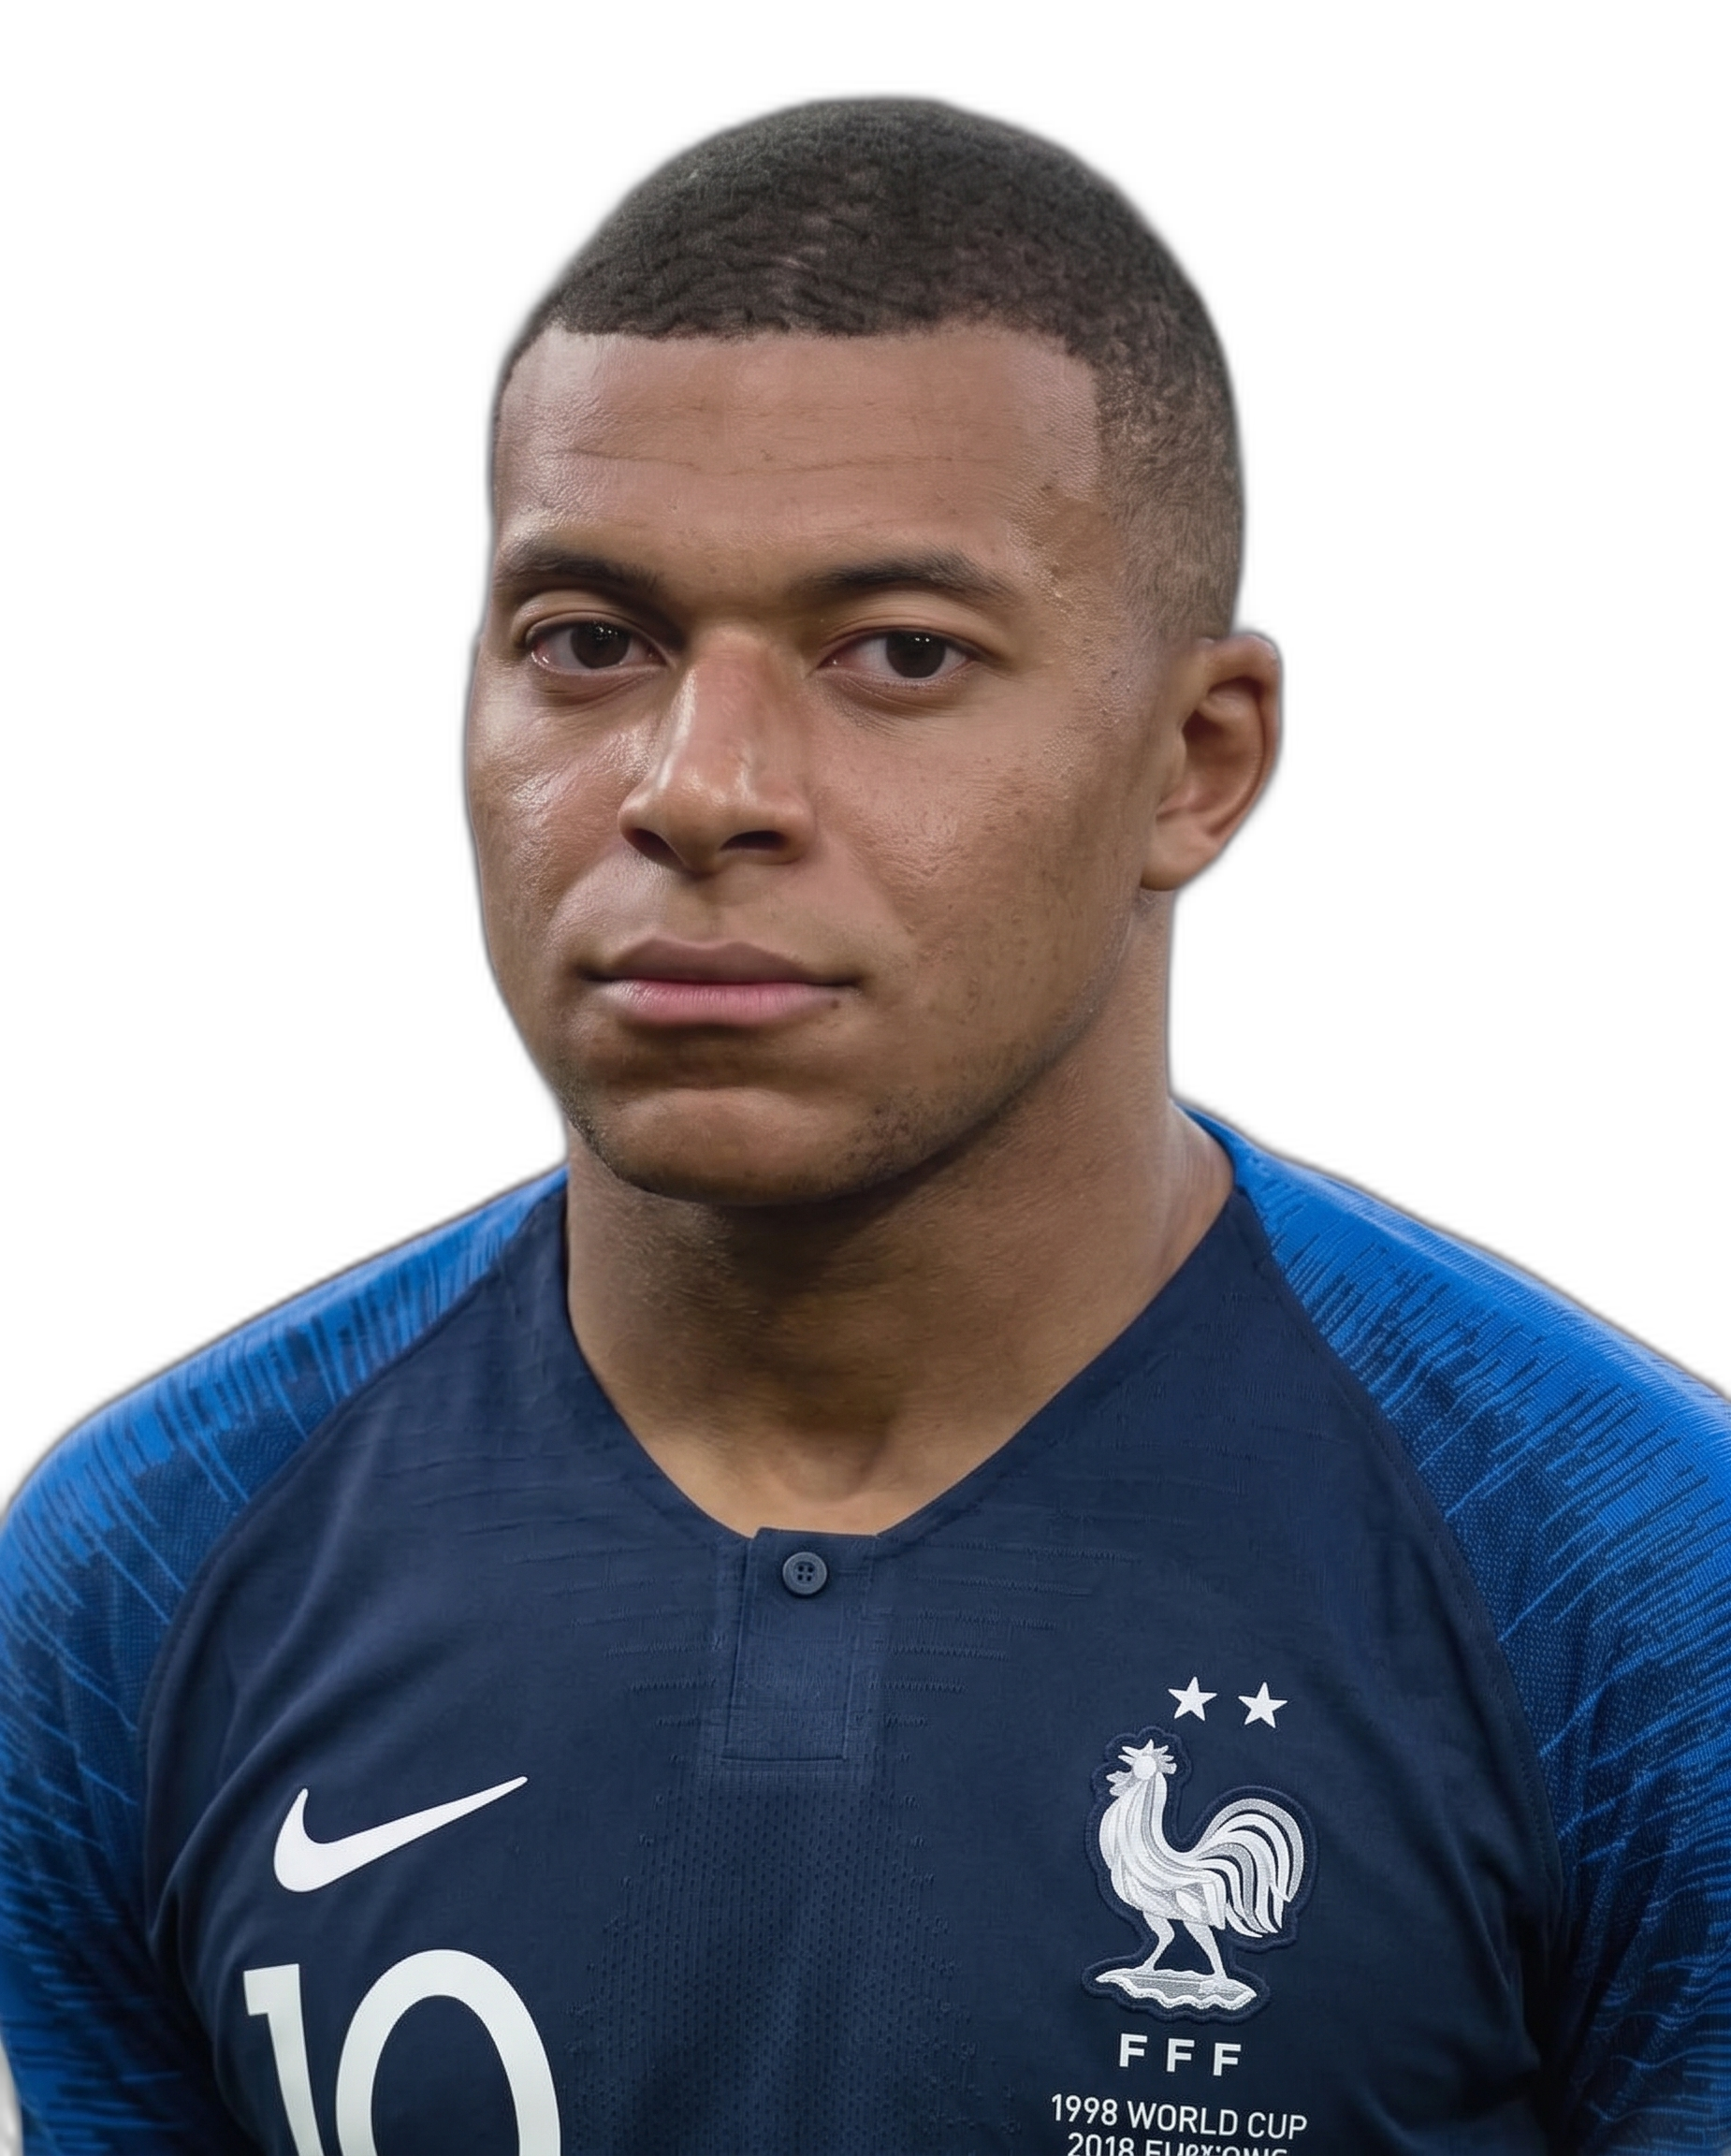
\includegraphics[height=7.6cm]{mbappe_before_cutout.png}};
  \node[anchor=south, inner sep=0pt, visible on=<3->] at (4.6, -4.5)
    {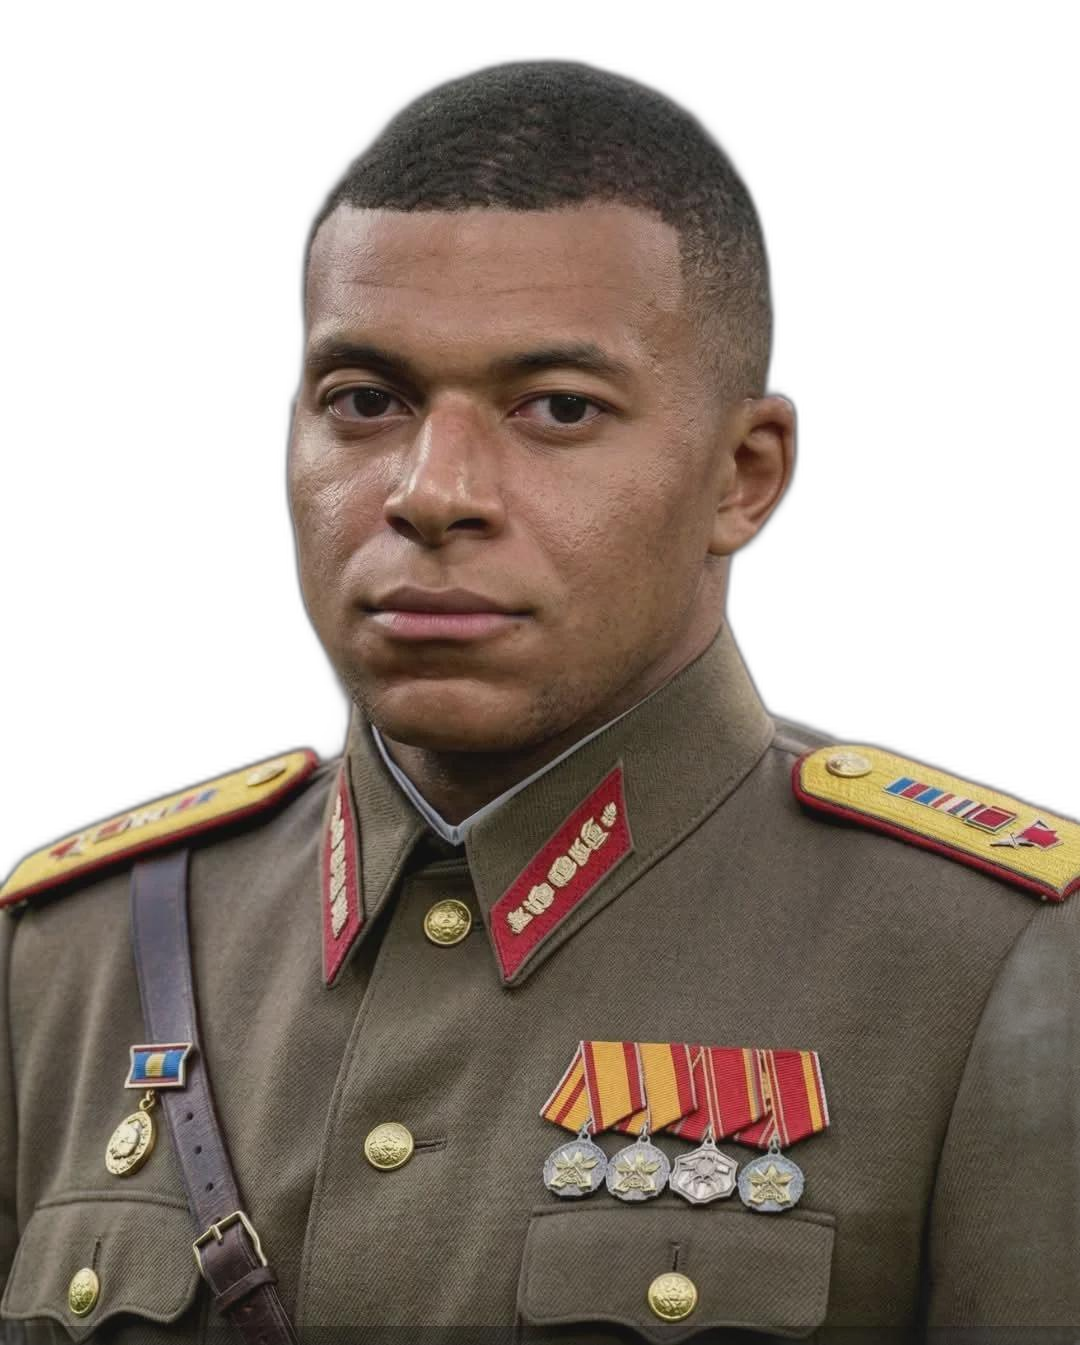
\includegraphics[height=7.6cm]{mbappe_after_cutout.png}};

  % 7. Network Badges around Mbappé on overlay 3
  \node[bankbadge, visible on=<3->] (bank) at ( 5.8, 2.7) {VERIFIED ALLY};
  \node[scambadge, visible on=<3->] (scamL) at ( 1.9, -1.4) {MILITARY REGIME};
  \node[scambadge, visible on=<3->] (scamR) at ( 6.2, -3.2) {SANCTIONED FACTION};

  % Crimson connection threads linking to Dictator Mbappé
  \draw[crimson, line width=1.6pt, visible on=<3->] (bank.south) -- (5.0, 0.4);
  \draw[crimson, line width=1.6pt, visible on=<3->] (scamL.east)  -- (3.4, -1.0);
  \draw[crimson, line width=1.6pt, visible on=<3->] (scamR.west)  -- (5.4, -1.8);

  % 8. Bottom Takeaway on overlay 4
  \node[visible on=<4->, anchor=south west, text=crimson, font=\fontsize{9.5}{12}\selectfont\twfont\bfseries, align=left]
    at (-7.2, -4.1) {ISOLATION FAILS\\CONNECTIONS REVEAL THE TRUTH};

\end{tikzpicture}
\end{frame}

% --- 1.3: Cold Open · The Core Pivot ---
\begin{frame}[plain]
\kicker{SCENE 01 / 17 \quad COLD OPEN}
\begin{tikzpicture}[remember picture,overlay,shift={(current page.center)}]

  % 1. Fluid organic wave backdrop on left (Warm paper/sand theme tone, NO GRID)
  \begin{scope}
    \clip (-8.5, -4.6) rectangle (3.0, 4.6);
    \fill[waveshape, draw=brass!40, line width=1.0pt] (-8.5, -4.6) -- (-8.5, 1.5)
      .. controls (-6.8, 0.6) and (-4.8, 0.8) .. (-3.0, 1.7)
      .. controls (-1.6, 2.4) and (-0.2, 2.3) .. (1.0, 1.2)
      .. controls (1.9, 0.3) and (2.3, -1.8) .. (2.5, -4.6) -- cycle;
  \end{scope}

  % 2. Glossy 3D accent sphere in top-left
  \shade[ball color=gold!85] (-6.8, 2.4) circle (0.36cm);
  \fill[white, opacity=0.6] (-6.9, 2.52) circle (0.09cm);

  % 3. Main header
  \node[anchor=south west, text=chalk, font=\fontsize{22}{26}\selectfont\sffamily\bfseries, align=left]
    at (-7.2, 2.85) {Can we trust this person?};

  % 4. Tilted Glassmorphic Card (DICTATOR state)
  \begin{scope}[shift={(-3.3, 0.2)}, rotate=4]
    \fill[black!12, rounded corners=12pt] (-3.15, -1.55) rectangle (3.15, 1.45);
    \fill[papercream, rounded corners=12pt, draw=brass!50, line width=1.2pt] (-3.1, -1.5) rectangle (3.1, 1.4);
    \fill[paperdark, rounded corners=10pt, opacity=0.45] (-3.1, -1.5) rectangle (3.1, -0.65);

    \node[anchor=north west, text=brass!90!ink, font=\fontsize{7}{8}\selectfont\twfont\bfseries]
      at (-2.8, 1.22) {DOSSIER $\cdot$ PROFILE \#10};
    \node[anchor=north east, text=crimson, font=\fontsize{7}{8}\selectfont\twfont\bfseries]
      at (2.8, 1.22) {FLAGGED};

    \node[anchor=north west, text=crimson, font=\dispfont\fontsize{28}{30}\selectfont\bfseries]
      at (-2.8, 0.95) {DICTATOR};

    % Divider cleanly below title
    \draw[ink!20, line width=0.5pt] (-2.8, -0.08) -- (2.8, -0.08);

    \node[anchor=north west, text=ink!85, font=\fontsize{7.5}{9.5}\selectfont\twfont]
      at (-2.8, -0.22) {REGIME: TOTALITARIAN \qquad STATUS: SANCTIONED};

    \node[anchor=center, text=crimson, font=\fontsize{8}{10}\selectfont\twfont\bfseries, align=center]
      at (0.0, -1.15) {HIGH-RISK NETWORK CONTEXT};
  \end{scope}

  % 5. Right side: Mbappé in Dictator Uniform
  \node[anchor=south, inner sep=0pt] at (4.6, -4.5)
    {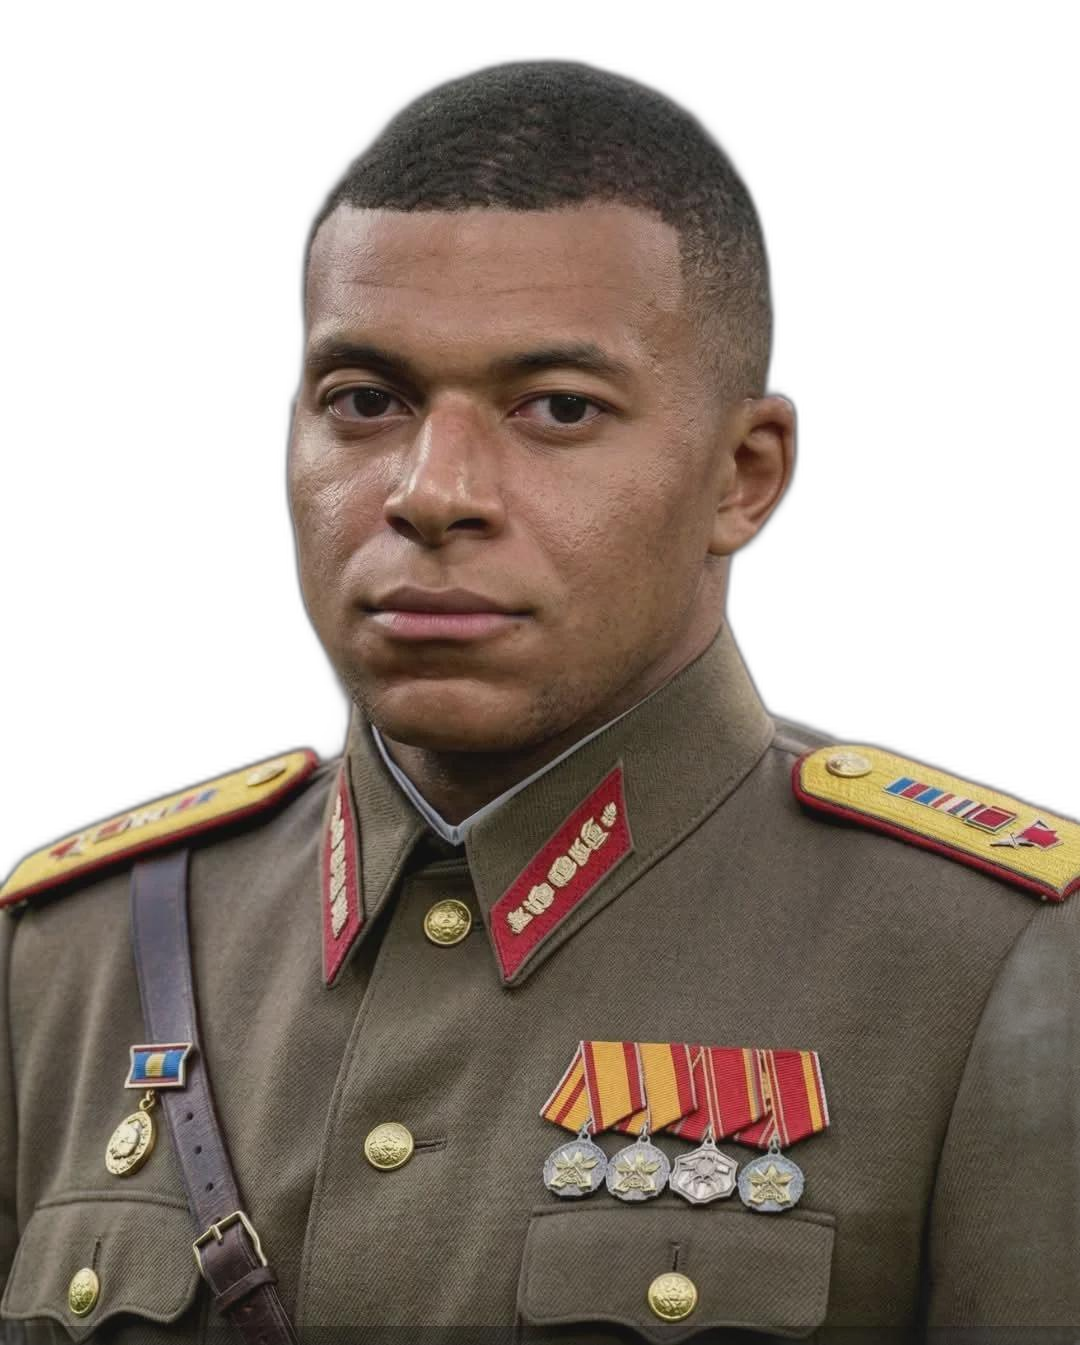
\includegraphics[height=7.6cm]{mbappe_after_cutout.png}};

  % 6. Network Badges around Mbappé
  \node[bankbadge] (bank) at ( 5.8, 2.7) {VERIFIED ALLY};
  \node[scambadge] (scamL) at ( 1.9, -1.4) {MILITARY REGIME};
  \node[scambadge] (scamR) at ( 6.2, -3.2) {SANCTIONED FACTION};

  % Crimson connection threads
  \draw[crimson, line width=1.6pt] (bank.south) -- (5.0, 0.4);
  \draw[crimson, line width=1.6pt] (scamL.east)  -- (3.4, -1.0);
  \draw[crimson, line width=1.6pt] (scamR.west)  -- (5.4, -1.8);

  % 7. The Core Pivot Questions on bottom left (clear of badges and portrait)
  \node[visible on=<2->, anchor=south west, text=chalk, font=\fontsize{15}{20}\selectfont\sffamily\bfseries, align=left]
    at (-7.2, -2.6) {What if the person itself\\isn't the information?};
  \node[visible on=<3->, anchor=south west, text=gold, font=\fontsize{18}{23}\selectfont\sffamily\bfseries, align=left]
    at (-7.2, -3.8) {What if the \underline{connections} are?};

\end{tikzpicture}
\end{frame}

% --- 2.1: CNN Example · Predictable Grid ---
\begin{frame}[plain]
\kicker{SCENE 02 / 17 \quad THE CNN EXAMPLE}
\begin{tikzpicture}[remember picture,overlay,shift={(current page.center)}]
  \foreach \r in {0,...,4} {
    \foreach \c in {0,...,4} {
      \fill[boardmid, draw=brass!25, line width=0.4pt, rounded corners=1pt]
        ({-2.4+\c*1.0}, {1.8-\r*1.0}) rectangle ({-2.4+\c*1.0+0.85}, {1.8-\r*1.0+0.85});
    }
  }
  \draw[gold, line width=2pt, rounded corners=2pt, visible on=<2->]
    (-1.45, -1.2) rectangle (1.5, 1.75);

  \node[visible on=<2->, anchor=north, text=gold, font=\fontsize{9}{10}\selectfont\twfont\bfseries]
    at (0, -1.5) {3$\times$3 CONVOLUTION PATCH};
  \node[visible on=<3->, anchor=north, text=brass, font=\fontsize{9}{11}\selectfont\twfont]
    at (0, -2.2) {LOCAL CONNECTIVITY $\cdot$ FIXED SPATIAL GRID};
\end{tikzpicture}
\end{frame}

% --- 2.2-2.3: CNN Example · The hierarchy builds one rung at a time ---
\begin{frame}[plain]
\kicker{SCENE 02 / 17 \quad THE CNN EXAMPLE}
\begin{tikzpicture}[remember picture,overlay,shift={(current page.center)}]
  \begin{scope}[shift={(-3.8,0.2)}]
    \foreach \r in {0,...,4} {
      \foreach \c in {0,...,4} {
        \fill[boardmid, draw=brass!25, line width=0.4pt, rounded corners=1pt]
          ({-1.8+\c*0.72}, {1.4-\r*0.72}) rectangle ({-1.8+\c*0.72+0.62}, {1.4-\r*0.72+0.62});
      }
    }
    \draw[gold, line width=1.5pt, rounded corners=2pt]
      (-1.1, -0.8) rectangle (1.1, 1.4);
    \node[anchor=north, text=brass, font=\fontsize{7.5}{9}\selectfont\twfont] at (0,-1.8)
      {\only<1-4>{LOCAL PATCHES}\only<5->{REGULAR PIXEL GRID}};
  \end{scope}

  \draw[dashed, dimtext!40, line width=0.5pt] (-0.8,-2.8) -- (-0.8,2.8);

  \node[draw=brass!50, fill=boardmid, text=chalk, rounded corners=2pt, minimum width=3.6cm,
        minimum height=0.55cm, font=\fontsize{8}{9}\selectfont\sffamily] (p) at (2.6, 2.0) {Pixels};
  \node[visible on=<2->, draw=brass!50, fill=boardmid, text=chalk, rounded corners=2pt, minimum width=3.6cm,
        minimum height=0.55cm, font=\fontsize{8}{9}\selectfont\sffamily] (e) at (2.6, 1.1) {Edges};
  \node[visible on=<3->, draw=brass!50, fill=boardmid, text=chalk, rounded corners=2pt, minimum width=3.6cm,
        minimum height=0.55cm, font=\fontsize{8}{9}\selectfont\sffamily] (pt) at (2.6, 0.2) {Patterns};
  \node[visible on=<4->, draw=brass!50, fill=boardmid, text=chalk, rounded corners=2pt, minimum width=3.6cm,
        minimum height=0.55cm, font=\fontsize{8}{9}\selectfont\sffamily] (sh) at (2.6, -0.7) {Shapes};
  \node[visible on=<5->, draw=gold, fill=boardmid, text=gold, line width=1.2pt, rounded corners=2pt,
        minimum width=3.6cm, minimum height=0.65cm, font=\fontsize{9}{10}\selectfont\sffamily\bfseries] (ob) at (2.6, -1.7) {Object Recognized};

  \draw[-{Latex[length=3pt]}, brass, visible on=<2->] (p) -- (e);
  \draw[-{Latex[length=3pt]}, brass, visible on=<3->] (e) -- (pt);
  \draw[-{Latex[length=3pt]}, brass, visible on=<4->] (pt) -- (sh);
  \draw[-{Latex[length=3pt]}, gold,  visible on=<5->] (sh) -- (ob);

  \node[visible on=<6->, anchor=south, text=gold, font=\fontsize{10}{12}\selectfont\twfont\bfseries, align=center]
    at (0,-3.3) {RIGID GEOMETRIC HIERARCHY};
\end{tikzpicture}
\end{frame}

% --- 3.1: Name the CNN ---
\begin{frame}[plain]
\kicker{SCENE 03 / 17 \quad NAME THE CNN}
\begin{tikzpicture}[remember picture,overlay,shift={(current page.center)}]
  \draw[brass, line width=0.8pt] (-5.5, 2.4) -- (5.5, 2.4);
  \node[anchor=center, text=chalk, font=\dispfont\fontsize{46}{42}\selectfont, align=center]
    at (0, 1.15) {Convolutional\\[-3pt]Neural Network};
  \node[visible on=<2->, draw=brass, fill=boardmid, text=brass, rounded corners=2pt,
        inner xsep=18pt, inner ysep=6pt, font=\dispfont\Large\bfseries] at (0,-0.85) {CNN};
  \node[visible on=<3->, anchor=center, text=dimtext, font=\fontsize{9}{11}\selectfont\twfont, align=center]
    at (0,-1.6) {BUILT FOR REGULAR EUCLIDEAN GRIDS};
  \draw[brass, line width=0.4pt] (-5.5,-2.3) -- (5.5,-2.3);
\end{tikzpicture}
\end{frame}

% --- 4.1-4.2: Grid vs Graph ---
\begin{frame}[plain]
\kicker{SCENE 04 / 17 \quad GRID VS.\ GRAPH}
\begin{tikzpicture}[remember picture,overlay,shift={(current page.center)}]
  \begin{scope}[shift={(-3.4, 0.4)}]
    \foreach \r in {0,...,4} {
      \foreach \c in {0,...,4} {
        \fill[boardmid, draw=brass!20, line width=0.3pt, rounded corners=1pt]
          ({-1.8+\c*0.82},{1.6-\r*0.82}) rectangle ({-1.8+\c*0.82+0.74},{1.6-\r*0.82+0.74});
      }
    }
    \foreach \r/\c in {1/2,3/2,2/1,2/3} {
      \fill[brass!25, draw=brass!60, line width=0.6pt, rounded corners=1pt, visible on=<2>]
        ({-1.8+\c*0.82},{1.6-\r*0.82}) rectangle ({-1.8+\c*0.82+0.74},{1.6-\r*0.82+0.74});
    }
    \fill[gold!30, draw=gold, line width=1.5pt, rounded corners=1pt]
      ({-1.8+2*0.82},{1.6-2*0.82}) rectangle ({-1.8+2*0.82+0.74},{1.6-2*0.82+0.74});
    \node[anchor=center, text=gold, font=\fontsize{7.5}{9}\selectfont\twfont\bfseries]
      at ({-1.8+2*0.82+0.37},{1.6-2*0.82+0.37}) {37};
    \node[visible on=<3->, anchor=north, text=dimtext, font=\fontsize{7.5}{9}\selectfont\twfont] at (0,-1.9) {REGULAR GRID};
  \end{scope}

  \draw[dashed, dimtext!40, line width=0.5pt] (0.0,-2.6) -- (0.0,2.6);

  \node[visible on=<2>, anchor=center, text=dimtext!60, font=\fontsize{14}{16}\selectfont\sffamily, align=center]
    at (3.4, 0.4) {What happens when the\\data has no grid?};

  \begin{scope}[shift={(3.4, 0.4)}]
    \coordinate (n1) at (-1.5, 1.2);
    \coordinate (n2) at ( 1.0, 0.8);
    \coordinate (n3) at ( 1.8,-0.5);
    \coordinate (n4) at ( 0.5,-1.3);
    \coordinate (n5) at (-1.6,-0.9);
    \coordinate (n6) at (-2.0, 0.1);

    \foreach \a/\b in {n1/n2, n2/n3, n3/n4, n4/n5, n5/n6, n6/n1, n1/n5, n2/n4} {
      \draw[gedge, visible on=<3->] (\a)--(\b);
    }
    \foreach \c in {n1,n2,n3,n4,n5,n6} {
      \node[gnode, visible on=<3->] at (\c) {};
    }
    \node[visible on=<3->, anchor=north, text=crimson!85, font=\fontsize{7.5}{9}\selectfont\twfont] at (0,-1.9) {IRREGULAR GRAPH};
  \end{scope}

  \node[visible on=<4->, anchor=south, text=gold, font=\fontsize{13}{15}\selectfont\sffamily\bfseries, align=center]
    at (0,-3.2) {There is no pixel 37.};
  \node[visible on=<4->, anchor=south, text=dimtext, font=\fontsize{8.5}{10}\selectfont\twfont, align=center]
    at (0,-3.7) {NO FIXED ORDER $\cdot$ ARBITRARY NEIGHBORS};
\end{tikzpicture}
\end{frame}

% --- 5.1-5.2: Two obvious solutions ---
\begin{frame}[plain]
\kicker{SCENE 05 / 17 \quad OBVIOUS SOLUTIONS}
\begin{tikzpicture}[remember picture,overlay,shift={(current page.center)}]
  \node[anchor=north, text=brass, font=\fontsize{9}{11}\selectfont\twfont\bfseries]
    at (-3.0, 2.5) {SOLUTION 1: DISCARD THE EDGES};

  \begin{scope}[shift={(-3.0, 0.5)}]
    \node[circle, draw=brass, fill=boardmid, minimum size=22pt] at (-1.4,  0.7) {};
    \node[circle, draw=brass, fill=boardmid, minimum size=22pt] at ( 0.8,  0.8) {};
    \node[circle, draw=brass, fill=boardmid, minimum size=22pt] at (-1.1, -0.9) {};
    \node[circle, draw=brass, fill=boardmid, minimum size=22pt] at ( 1.2, -0.6) {};
    \node[visible on=<2->, anchor=north, text=crimson, font=\fontsize{8}{10}\selectfont\twfont\bfseries]
      at (0,-1.4) {LOSES GRAPH STRUCTURE};
  \end{scope}

  \draw[dashed, dimtext!40, line width=0.5pt] (0.0,-2.6) -- (0.0,2.6);

  \node[visible on=<2>, anchor=center, text=dimtext!60, font=\fontsize{12}{14}\selectfont\sffamily]
    at (3.0, 0.5) {What if we keep them?};

  \node[visible on=<3->, anchor=north, text=brass, font=\fontsize{9}{11}\selectfont\twfont\bfseries]
    at (3.0, 2.5) {SOLUTION 2: ADJACENCY MATRIX};

  \begin{scope}[shift={(3.0, 0.5)}]
    \fill[papercream, rounded corners=3pt, visible on=<3->] (-2.2,-1.6) rectangle (2.2,1.3);
    \node[visible on=<3->, anchor=north, text=ink, font=\fontsize{8}{9}\selectfont\twfont\bfseries]
      at (0, 1.1) {Adjacency Matrix $A$};
    \node[visible on=<3->, anchor=center, text=ink, font=\fontsize{8}{11}\selectfont\ttfamily] at (0, -0.15) {
      $\begin{bmatrix}
        0 & 1 & 0 & 1 \\
        1 & 0 & 1 & 0 \\
        0 & 1 & 0 & 1 \\
        1 & 0 & 1 & 0
      \end{bmatrix}$
    };
    \node[visible on=<4->, anchor=north, text=crimson, font=\fontsize{8}{10}\selectfont\twfont\bfseries]
      at (0,-1.15) {SENSITIVE TO NODE ORDERING};
  \end{scope}

  \node[visible on=<5->, anchor=south, text=gold, font=\fontsize{12}{14}\selectfont\sffamily\bfseries, align=center]
    at (0,-3.4) {Why do naive approaches fail?};
\end{tikzpicture}
\end{frame}

% --- 6.1-6.2: The Failure · Renumber the same molecule ---
\begin{frame}[plain]
\kicker{SCENE 06 / 17 \quad THE FAILURE}
\begin{tikzpicture}[remember picture,overlay,shift={(current page.center)}]
  \node[anchor=north, text=chalk, font=\fontsize{12}{14}\selectfont\sffamily\bfseries]
    at (0, 2.6) {Same molecule. Same atoms. Same bonds.};

  \begin{scope}[shift={(-3.2, 0.2)}]
    \node[anchor=north, text=brass, font=\fontsize{8}{9}\selectfont\twfont\bfseries] at (0, 1.8) {NUMBERING A};
    \coordinate (a1) at ( 0.0, 1.0);
    \coordinate (a2) at (-1.1, 0.5);
    \coordinate (a3) at (-1.1,-0.6);
    \coordinate (a4) at ( 0.0,-1.1);
    \coordinate (a5) at ( 1.1,-0.6);
    \coordinate (a6) at ( 1.1, 0.5);
    \draw[gedge] (a1)--(a2)--(a3)--(a4)--(a5)--(a6)--(a1);
    \draw[gedge] (a1)--(a4);
    \foreach \n/\coord in {1/a1, 2/a2, 3/a3, 4/a4, 5/a5, 6/a6} {
      \node[circle, draw=brass, fill=boardmid, text=chalk, font=\fontsize{7}{8}\selectfont\twfont, inner sep=1pt] at (\coord) {\n};
    }
    \fill[papercream, rounded corners=2pt, visible on=<2->] (-1.6,-2.2) rectangle (1.6,-1.4);
    \node[visible on=<2->, anchor=center, text=biogreen!80!ink, font=\fontsize{9}{10}\selectfont\twfont\bfseries] at (0, -1.8) {Toxicity: 0.83};
  \end{scope}

  \draw[dashed, dimtext!40, line width=0.5pt] (0.0,-2.4) -- (0.0,2.1);

  \node[visible on=<3>, anchor=center, text=dimtext!60, font=\fontsize{11}{13}\selectfont\sffamily, align=center]
    at (3.2, 0.2) {What if we simply\\renumber the atoms?};

  \begin{scope}[shift={(3.2, 0.2)}]
    \node[visible on=<4->, anchor=north, text=brass, font=\fontsize{8}{9}\selectfont\twfont\bfseries] at (0, 1.8) {NUMBERING B};
    \coordinate (b1) at ( 0.0, 1.0);
    \coordinate (b2) at (-1.1, 0.5);
    \coordinate (b3) at (-1.1,-0.6);
    \coordinate (b4) at ( 0.0,-1.1);
    \coordinate (b5) at ( 1.1,-0.6);
    \coordinate (b6) at ( 1.1, 0.5);
    \draw[gedge, visible on=<4->] (b1)--(b2)--(b3)--(b4)--(b5)--(b6)--(b1);
    \draw[gedge, visible on=<4->] (b1)--(b4);
    \foreach \n/\coord in {4/b1, 1/b2, 6/b3, 2/b4, 5/b5, 3/b6} {
      \node[visible on=<4->, circle, draw=brass, fill=boardmid, text=chalk, font=\fontsize{7}{8}\selectfont\twfont, inner sep=1pt] at (\coord) {\n};
    }
    \fill[papercream, rounded corners=2pt, visible on=<5->] (-1.6,-2.2) rectangle (1.6,-1.4);
    \node[visible on=<5->, anchor=center, text=crimson, font=\fontsize{9}{10}\selectfont\twfont\bfseries] at (0, -1.8) {Toxicity: 0.11};
  \end{scope}

  \node[visible on=<6->, anchor=south, text=crimson, font=\fontsize{9.5}{11}\selectfont\twfont\bfseries, align=center]
    at (0,-3.3) {PERMUTATION SENSITIVITY $\cdot$ ARBITRARY NUMBERING BIAS};
\end{tikzpicture}
\end{frame}

% --- 6.3: The Failure · The Red X Stamp ---
\begin{frame}[plain]
\kicker{SCENE 06 / 17 \quad THE FAILURE}
\begin{tikzpicture}[remember picture,overlay,shift={(current page.center)}]
  \begin{scope}[shift={(-3.2, 0.5)}]
    \node[anchor=north, text=brass, font=\fontsize{8}{9}\selectfont\twfont] at (0, 1.6) {NUMBERING A};
    \fill[papercream, rounded corners=2pt] (-1.6,-1.4) rectangle (1.6,-0.7);
    \node[anchor=center, text=biogreen!80!ink, font=\fontsize{9}{10}\selectfont\twfont\bfseries] at (0, -1.05) {Toxicity: 0.83};
  \end{scope}

  \begin{scope}[shift={(3.2, 0.5)}]
    \node[anchor=north, text=brass, font=\fontsize{8}{9}\selectfont\twfont] at (0, 1.6) {NUMBERING B};
    \fill[papercream, rounded corners=2pt] (-1.6,-1.4) rectangle (1.6,-0.7);
    \node[anchor=center, text=crimson, font=\fontsize{9}{10}\selectfont\twfont\bfseries] at (0, -1.05) {Toxicity: 0.11};
    \draw[crimson, line width=6pt, cap=round, visible on=<2->] (-2.2, 1.4) -- (2.2, -1.4);
    \draw[crimson, line width=6pt, cap=round, visible on=<2->] (-2.2, -1.4) -- (2.2, 1.4);
  \end{scope}

  \node[visible on=<3->, anchor=north, text=gold, font=\fontsize{15}{18}\selectfont\sffamily\bfseries, align=center]
    at (0, -1.6) {The network learned our filing system.};
  \node[visible on=<4->, anchor=north, text=chalk, font=\fontsize{15}{18}\selectfont\sffamily\bfseries, align=center]
    at (0, -2.3) {It never learned the chemistry.};
\end{tikzpicture}
\end{frame}

% =============================================================
% ACT II: THE MECHANISM
% =============================================================

% --- 7.1-7.2: The Pivotal Question · One word changes the problem ---
\begin{frame}[plain]
\kicker{SCENE 07 / 17 \quad THE PIVOTAL QUESTION}
\begin{tikzpicture}[remember picture,overlay,shift={(current page.center)}]
  \node[visible on=<1>, anchor=south, text=chalk, font=\fontsize{22}{26}\selectfont\sffamily\bfseries]
    at (0, 1.9) {What \textbf{is} this node?};
  \node[visible on=<2->, anchor=south, text=chalk!70, font=\fontsize{18}{22}\selectfont\sffamily]
    at (0, 1.95) {What \sout{\textcolor{crimson}{is}} this node?};

  \foreach \r/\op in {1.8/0.08, 1.3/0.15, 0.85/0.25} {
    \fill[gold, opacity=\op, visible on=<3->] (0, 0.3) circle (\r cm);
  }
  \node[circle, draw=gold, fill=boardmid, line width=2.5pt, minimum size=32pt] at (0, 0.3) {};

  \node[visible on=<3->, anchor=north, text=gold, font=\fontsize{22}{26}\selectfont\sffamily\bfseries]
    at (0, -1.0) {Who \underline{influences} this node?};

  \node[visible on=<4->, anchor=north, text=brass, font=\fontsize{11}{13}\selectfont\twfont\bfseries, align=center]
    at (0, -2.0) {RELATIONAL REASONING};
\end{tikzpicture}
\end{frame}

% --- 8.1-8.4: The GNN Idea · Gather, Aggregate, Update in one place ---
\begin{frame}[plain]
\kicker{SCENE 08 / 17 \quad THE GNN IDEA}
\begin{tikzpicture}[remember picture,overlay,shift={(current page.center)}]
  \coordinate (c)  at ( 0.0,  0.7);
  \coordinate (n1) at (-3.2,  2.4);
  \coordinate (n2) at ( 3.2,  2.4);
  \coordinate (n3) at ( 0.0, -1.4);

  % Edges: calm on overlay 1 and 3-, hot while gathering
  \draw[gedge, visible on=<1>]   (n1) -- (c);
  \draw[gedge, visible on=<1>]   (n2) -- (c);
  \draw[gedge, visible on=<1>]   (n3) -- (c);
  \draw[gedge, visible on=<3->]  (n1) -- (c);
  \draw[gedge, visible on=<3->]  (n2) -- (c);
  \draw[gedge, visible on=<3->]  (n3) -- (c);
  \draw[gedgeHot, -{Latex[length=6pt]}, visible on=<2>] (n1) -- (c);
  \draw[gedgeHot, -{Latex[length=6pt]}, visible on=<2>] (n2) -- (c);
  \draw[gedgeHot, -{Latex[length=6pt]}, visible on=<2>] (n3) -- (c);

  % Envelopes mid-flight during GATHER
  \fill[gold, visible on=<2>] (-1.6,1.55) ++(-0.25,-0.15) rectangle +(0.5,0.3);
  \draw[ink, line width=0.5pt, visible on=<2>] (-1.6-0.25,1.55+0.15) -- (-1.6,1.55) -- (-1.6+0.25,1.55+0.15);
  \fill[gold, visible on=<2>] (1.6,1.55) ++(-0.25,-0.15) rectangle +(0.5,0.3);
  \draw[ink, line width=0.5pt, visible on=<2>] (1.6-0.25,1.55+0.15) -- (1.6,1.55) -- (1.6+0.25,1.55+0.15);
  \fill[gold, visible on=<2>] (0.0,-0.35) ++(-0.25,-0.15) rectangle +(0.5,0.3);
  \draw[ink, line width=0.5pt, visible on=<2>] (0.0-0.25,-0.35+0.15) -- (0.0,-0.35) -- (0.0+0.25,-0.35+0.15);

  \node[gnode] at (n1) {};
  \node[gnode] at (n2) {};
  \node[gnode] at (n3) {};
  \node[visible on=<1-3>, gnodeFocus, minimum size=34pt] at (c) {};
  \node[visible on=<4->, circle, draw=gold, fill=gold!30, line width=2.5pt, minimum size=34pt] at (c) {};

  % The aggregation box appears inside the target on step 2
  \fill[gold, visible on=<3>] (-0.35, 0.55) rectangle (0.35, 0.85);
  \node[visible on=<3>, anchor=center, text=ink, font=\fontsize{6.5}{7}\selectfont\twfont\bfseries] at (0, 0.7) {$\sum$};

  % Step chips light up one at a time and stay on the board
  \begin{scope}[shift={(0, -2.7)}]
    \node[visible on=<1>,   gstep]   (g1a) at (-3.4,0) {\textbf{1.} GATHER};
    \node[visible on=<2->,  gstepon] (g1)  at (-3.4,0) {\textbf{1.} GATHER};
    \node[visible on=<1-2>, gstep]   (g2a) at ( 0.0,0) {\textbf{2.} AGGREGATE};
    \node[visible on=<3->,  gstepon] (g2)  at ( 0.0,0) {\textbf{2.} AGGREGATE};
    \node[visible on=<1-3>, gstep]   (g3a) at ( 3.4,0) {\textbf{3.} UPDATE};
    \node[visible on=<4->,  gstepon] (g3)  at ( 3.4,0) {\textbf{3.} UPDATE};
    \draw[-{Latex[length=4pt]}, brass!60] (g1a)--(g2a);
    \draw[-{Latex[length=4pt]}, brass!60] (g2a)--(g3a);
  \end{scope}

  \node[visible on=<5->, anchor=north, text=gold, font=\fontsize{11}{13}\selectfont\twfont\bfseries, align=center]
    at (0,-3.4) {MESSAGE PASSING MECHANISM};
\end{tikzpicture}
\end{frame}

% =============================================================
% ACT II-A: RUN ONE LAYER BY HAND (ALICE'S GRAPH, REAL NUMBERS)
% =============================================================

% --- 9.0: The data on the table ---
\begin{frame}[plain]
\kicker{SCENE 09 / 17 \quad RUN IT BY HAND $\cdot$ SETUP}
\begin{tikzpicture}[remember picture,overlay,shift={(current page.center)}]
  \node[anchor=north, text=chalk, font=\fontsize{12.5}{15}\selectfont\sffamily\bfseries]
    at (0, 3.85) {Is Alice likely to be interested in Topic X?};

  % ---------- the graph (left) ----------
  \begin{scope}[shift={(-4.05, 0.15)}]
    \draw[gedge] (0,0) -- (-2.2,1.9);
    \draw[gedge] (0,0) -- ( 2.2,1.9);
    \draw[gedge] (-2.2,1.9) -- (-2.5,-1.9);
    \draw[gedge] ( 2.2,1.9) -- ( 2.5,-1.9);

    \node[pcard] at (-2.2, 1.9) {\pbody{Bob}{0.60}{1.00}{biogreen!70!ink}};
    \node[pcard] at ( 2.2, 1.9) {\pbody{Carol}{0.40}{1.00}{biogreen!70!ink}};
    \node[pcard] at (-2.5,-1.9) {\pbody{David}{0.20}{0.00}{ink!55}};
    \node[pcard] at ( 2.5,-1.9) {\pbody{Eve}{0.80}{0.00}{ink!55}};
    \node[pcardHot] at (0,0) {\pbody{ALICE}{0.80}{0.00}{crimson}};

    \node[visible on=<4->, anchor=north, text=crimson, font=\fontsize{6.5}{8}\selectfont\twfont\bfseries]
      at (0,-0.78) {TOPIC X UNKNOWN};
  \end{scope}

  % ---------- the worksheet (right) ----------
  \draw[sheet] (0.0,-3.45) rectangle (7.6, 3.0);

  \node[shead] at (0.3, 2.78) {THE DATA};


  \node[visible on=<2->, shead]    at (0.3, 1.62) {SLOT 1 \quad ACTIVITY};
  \node[visible on=<2->, slineDim] at (0.65, 1.30) {how much they post};
  \node[visible on=<2->, slineDim] at (0.65, 1.02) {0 = never \quad 1 = constantly};
  \node[visible on=<2->, shead]    at (0.3, 0.62) {SLOT 2 \quad TOPIC X};
  \node[visible on=<2->, slineDim] at (0.65, 0.30) {how much they engage with Topic X};
  \node[visible on=<2->, slineDim] at (0.65, 0.02) {0 = never \quad 1 = all the time};

  \node[visible on=<3->, shead] at (0.3,-0.44) {THE FIVE CARDS};
  \node[visible on=<3->, sline] at (0.65,-0.80) {Bob \ \ \ [ 0.60 , 1.00 ]};
  \node[visible on=<3->, sline] at (0.65,-1.10) {Carol \ [ 0.40 , 1.00 ]};
  \node[visible on=<3->, sline] at (0.65,-1.40) {David \ [ 0.20 , 0.00 ]};
  \node[visible on=<3->, sline] at (0.65,-1.70) {Eve \ \ \ [ 0.80 , 0.00 ]};
  \node[visible on=<3->, slineHot] at (0.65,-2.02) {Alice \ [ 0.80 , 0.00 ]};



  % ---------- progress strip ----------
  \node[gstep] at (-2.6,-3.95) {1. GATHER};
  \node[gstep] at ( 0.0,-3.95) {2. AGGREGATE};
  \node[gstep] at ( 2.6,-3.95) {3. UPDATE};
  \node[visible on=<5->, anchor=center, text=gold, font=\fontsize{8}{10}\selectfont\twfont\bfseries]
    at (5.3,-3.95) {= ONE LAYER};
\end{tikzpicture}
\end{frame}

% --- 9.1: STEP 1 - GATHER ---
\begin{frame}[plain]
\kicker{SCENE 09 / 17 \quad RUN IT BY HAND $\cdot$ STEP 1}
\begin{tikzpicture}[remember picture,overlay,shift={(current page.center)}]
  \node[anchor=north, text=chalk, font=\fontsize{12.5}{15}\selectfont\sffamily\bfseries]
    at (0, 3.85) {Step 1 of 3 --- \textcolor{gold}{GATHER}};

  \begin{scope}[shift={(-4.05, 0.15)}]
    \draw[gedge, visible on=<1>] (0,0) -- (-2.2,1.9);
    \draw[gedge, visible on=<1>] (0,0) -- ( 2.2,1.9);
    \draw[gedgeHot, -{Latex[length=6pt]}, visible on=<2->] (-2.2,1.9) -- (0,0);
    \draw[gedgeHot, -{Latex[length=6pt]}, visible on=<2->] ( 2.2,1.9) -- (0,0);
    \draw[gedge,    visible on=<1-2>] (-2.2,1.9) -- (-2.5,-1.9);
    \draw[gedge,    visible on=<1-2>] ( 2.2,1.9) -- ( 2.5,-1.9);
    \draw[gedgeDim, visible on=<3->]  (-2.2,1.9) -- (-2.5,-1.9);
    \draw[gedgeDim, visible on=<3->]  ( 2.2,1.9) -- ( 2.5,-1.9);

    \node[visible on=<1>,   pcard]    at (-2.2, 1.9) {\pbody{Bob}{0.60}{1.00}{biogreen!70!ink}};
    \node[visible on=<2->,  pcardHot] at (-2.2, 1.9) {\pbody{Bob}{0.60}{1.00}{biogreen!70!ink}};
    \node[visible on=<1>,   pcard]    at ( 2.2, 1.9) {\pbody{Carol}{0.40}{1.00}{biogreen!70!ink}};
    \node[visible on=<2->,  pcardHot] at ( 2.2, 1.9) {\pbody{Carol}{0.40}{1.00}{biogreen!70!ink}};
    \node[visible on=<1-2>, pcard]    at (-2.5,-1.9) {\pbody{David}{0.20}{0.00}{ink!55}};
    \node[visible on=<3->,  pcardDim] at (-2.5,-1.9) {\pbody{David}{0.20}{0.00}{ink!60}};
    \node[visible on=<1-2>, pcard]    at ( 2.5,-1.9) {\pbody{Eve}{0.80}{0.00}{ink!55}};
    \node[visible on=<3->,  pcardDim] at ( 2.5,-1.9) {\pbody{Eve}{0.80}{0.00}{ink!60}};
    \node[pcardHot] at (0,0) {\pbody{ALICE}{0.80}{0.00}{crimson}};

    \node[visible on=<4->, fill=gold, text=ink, rounded corners=2pt, inner xsep=3pt, inner ysep=2pt,
          font=\fontsize{6.5}{7.5}\selectfont\twfont\bfseries] at (-1.1, 0.95) {0.60 , 1.00};
    \node[visible on=<5->, fill=gold, text=ink, rounded corners=2pt, inner xsep=3pt, inner ysep=2pt,
          font=\fontsize{6.5}{7.5}\selectfont\twfont\bfseries] at ( 1.1, 0.95) {0.40 , 1.00};
  \end{scope}

  \draw[sheet] (0.0,-3.45) rectangle (7.6, 3.0);

  \node[shead] at (0.3, 2.78) {STEP 1 \quad GATHER};


  \node[visible on=<2->, slineHot] at (0.3, 1.62) {N(Alice) = \{ Bob , Carol \}};



  \node[visible on=<4->, shead] at (0.3, 0.40) {WHAT IS A MESSAGE?};


  \node[visible on=<4->, sline] at (0.65,-0.74) {Bob \ \ sends \ [ 0.60 , 1.00 ]};
  \node[visible on=<5->, sline] at (0.65,-1.04) {Carol sends \ [ 0.40 , 1.00 ]};

  \node[visible on=<6->, slineHot] at (0.3,-2.20) {Gathering = Copying messages};

  \node[gstepon] at (-2.6,-3.95) {1. GATHER};
  \node[gstep]   at ( 0.0,-3.95) {2. AGGREGATE};
  \node[gstep]   at ( 2.6,-3.95) {3. UPDATE};
\end{tikzpicture}
\end{frame}

% --- 9.2: STEP 2 - AGGREGATE ---
\begin{frame}[plain]
\kicker{SCENE 09 / 17 \quad RUN IT BY HAND $\cdot$ STEP 2}
\begin{tikzpicture}[remember picture,overlay,shift={(current page.center)}]
  \node[anchor=north, text=chalk, font=\fontsize{12.5}{15}\selectfont\sffamily\bfseries]
    at (0, 3.85) {Step 2 of 3 --- \textcolor{gold}{AGGREGATE}};

  \begin{scope}[shift={(-4.05, 0.15)}]
    \draw[gedgeHot, -{Latex[length=6pt]}] (-2.2,1.9) -- (0,0);
    \draw[gedgeHot, -{Latex[length=6pt]}] ( 2.2,1.9) -- (0,0);
    \draw[gedgeDim] (-2.2,1.9) -- (-2.5,-1.9);
    \draw[gedgeDim] ( 2.2,1.9) -- ( 2.5,-1.9);

    \node[pcardHot] at (-2.2, 1.9) {\pbody{Bob}{0.60}{1.00}{biogreen!70!ink}};
    \node[pcardHot] at ( 2.2, 1.9) {\pbody{Carol}{0.40}{1.00}{biogreen!70!ink}};
    \node[pcardDim] at (-2.5,-1.9) {\pbody{David}{0.20}{0.00}{ink!60}};
    \node[pcardDim] at ( 2.5,-1.9) {\pbody{Eve}{0.80}{0.00}{ink!60}};
    \node[pcardHot] at (0,0) {\pbody{ALICE}{0.80}{0.00}{crimson}};

    \node[visible on=<6->, draw=gold, fill=gold!25, text=ink, rounded corners=2pt, line width=1.2pt,
          inner xsep=5pt, inner ysep=3pt, align=center,
          font=\fontsize{6.5}{8}\selectfont\twfont\bfseries]
      at (0,-1.22) {NEIGHBOURHOOD\\[1pt][ 0.50 , 1.00 ]};
  \end{scope}

  \draw[sheet] (0.0,-3.45) rectangle (7.6, 3.0);

  \node[shead] at (0.3, 2.78) {STEP 2 \quad AGGREGATE};


  \node[visible on=<2->, sline] at (0.65, 1.62) {Bob \ \ \ [ 0.60 , 1.00 ]};
  \node[visible on=<2->, sline] at (0.65, 1.32) {Carol \ [ 0.40 , 1.00 ]};

  \node[visible on=<3->, slineHot] at (0.3, 0.86) {Rule: average them, slot by slot.};

  \node[visible on=<4->, sline] at (0.65, 0.38) {ACTIVITY \ (0.60 + 0.40) / 2 = 0.50};
  \node[visible on=<5->, sline] at (0.65, 0.03) {TOPIC X \ \ (1.00 + 1.00) / 2 = 1.00};

  \node[visible on=<6->, slineHot] at (0.3,-0.50) {m(Alice) = [ 0.50 , 1.00 ]};

  \node[visible on=<7->, shead] at (0.3,-1.08) {ORDER INVARIANCE};
  \node[visible on=<7->, slineHot] at (0.3,-1.50) {mean(Bob, Carol) = mean(Carol, Bob) = 0.50};

  \node[visible on=<8->, slineHot] at (0.3,-2.00) {Order Invariant Aggregation};



  \node[gstep]   at (-2.6,-3.95) {1. GATHER};
  \node[gstepon] at ( 0.0,-3.95) {2. AGGREGATE};
  \node[gstep]   at ( 2.6,-3.95) {3. UPDATE};
\end{tikzpicture}
\end{frame}

% --- 9.3: STEP 3 - UPDATE ---
\begin{frame}[plain]
\kicker{SCENE 09 / 17 \quad RUN IT BY HAND $\cdot$ STEP 3}
\begin{tikzpicture}[remember picture,overlay,shift={(current page.center)}]
  \node[anchor=north, text=chalk, font=\fontsize{12.5}{15}\selectfont\sffamily\bfseries]
    at (0, 3.85) {Step 3 of 3 --- \textcolor{gold}{UPDATE}};

  \begin{scope}[shift={(-4.05, 0.15)}]
    \draw[gedgeHot] (-2.2,1.9) -- (0,0);
    \draw[gedgeHot] ( 2.2,1.9) -- (0,0);
    \draw[gedgeDim] (-2.2,1.9) -- (-2.5,-1.9);
    \draw[gedgeDim] ( 2.2,1.9) -- ( 2.5,-1.9);

    \node[pcardHot] at (-2.2, 1.9) {\pbody{Bob}{0.60}{1.00}{biogreen!70!ink}};
    \node[pcardHot] at ( 2.2, 1.9) {\pbody{Carol}{0.40}{1.00}{biogreen!70!ink}};
    \node[pcardDim] at (-2.5,-1.9) {\pbody{David}{0.20}{0.00}{ink!60}};
    \node[pcardDim] at ( 2.5,-1.9) {\pbody{Eve}{0.80}{0.00}{ink!60}};

    \node[visible on=<1-6>, pcardHot] at (0,0) {\pbody{ALICE}{0.80}{0.00}{crimson}};
    \node[visible on=<7->, pcardHot, fill=gold!35] at (0,0) {\pbody{ALICE}{0.65}{0.50}{biogreen!65!ink}};

    \node[visible on=<1-6>, draw=gold, fill=gold!25, text=ink, rounded corners=2pt, line width=1.2pt,
          inner xsep=5pt, inner ysep=3pt, align=center,
          font=\fontsize{6.5}{8}\selectfont\twfont\bfseries]
      at (0,-1.22) {NEIGHBOURHOOD\\[1pt][ 0.50 , 1.00 ]};
    \node[visible on=<7->, anchor=north, text=gold, font=\fontsize{6.5}{8}\selectfont\twfont\bfseries]
      at (0,-0.78) {CARD REWRITTEN};
  \end{scope}

  \draw[sheet] (0.0,-3.45) rectangle (7.6, 3.0);

  \node[shead] at (0.3, 2.78) {STEP 3 \quad UPDATE};


  \node[visible on=<2->, sline] at (0.65, 1.62) {mine \ \ \ [ 0.80 , 0.00 ]};
  \node[visible on=<2->, sline] at (0.65, 1.32) {theirs \ [ 0.50 , 1.00 ]};

  \node[visible on=<3->, slineHot] at (0.3, 0.86) {new = 0.5 x mine + 0.5 x theirs};


  \node[visible on=<4->, sline] at (0.65,-0.52) {ACTIVITY \ 0.5(0.80) + 0.5(0.50)};
  \node[visible on=<4->, sline] at (0.65,-0.82) {\ \ \ \ \ \ \ \ \ = 0.40 + 0.25 = 0.65};

  \node[visible on=<5->, sline] at (0.65,-1.24) {TOPIC X \ \ 0.5(0.00) + 0.5(1.00)};
  \node[visible on=<5->, sline] at (0.65,-1.54) {\ \ \ \ \ \ \ \ \ = 0.00 + 0.50 = 0.50};



  \node[visible on=<7->, slineHot] at (0.3,-3.04) {h'(Alice) = [ 0.65 , 0.50 ]};

  \node[gstep]   at (-2.6,-3.95) {1. GATHER};
  \node[gstep]   at ( 0.0,-3.95) {2. AGGREGATE};
  \node[gstepon] at ( 2.6,-3.95) {3. UPDATE};
\end{tikzpicture}
\end{frame}

% --- 9.4: What that one number bought us ---
\begin{frame}[plain]
\kicker{SCENE 09 / 17 \quad RUN IT BY HAND $\cdot$ THE ANSWER}
\begin{tikzpicture}[remember picture,overlay,shift={(current page.center)}]
  \node[anchor=north, text=chalk, font=\fontsize{12.5}{15}\selectfont\sffamily\bfseries]
    at (0, 3.9) {One blank slot, filled in by the neighbourhood.};

  \node[anchor=north, text=brass, font=\fontsize{7.5}{9}\selectfont\twfont\bfseries] at (-3.4, 2.75) {BEFORE};
  \node[pcard, minimum width=2.4cm] at (-3.4, 1.8) {\pbody{ALICE}{0.80}{0.00}{crimson}};

  \draw[-{Latex[length=7pt]}, gold, line width=2pt, visible on=<2->] (-1.9, 1.8) -- (-0.5, 1.8);

  \node[visible on=<2->, anchor=north, text=gold, font=\fontsize{7.5}{9}\selectfont\twfont\bfseries] at (1.0, 2.75) {AFTER ONE LAYER};
  \node[visible on=<2->, pcardHot, fill=gold!35, minimum width=2.4cm] at (1.0, 1.8) {\pbody{ALICE}{0.65}{0.50}{biogreen!65!ink}};

  \node[visible on=<2->, anchor=west, text=chalk, font=\fontsize{10}{12}\selectfont\sffamily, align=left]
    at (2.8, 1.8) {TOPIC X: \ \textcolor{crimson}{0.00} $\rightarrow$ \textcolor{gold}{\bfseries 0.50}};

  \node[visible on=<3->, anchor=north, text=dimtext, font=\fontsize{8.5}{10}\selectfont\twfont\bfseries, align=center]
    at (0, -0.1) {READOUT LAYER};
  \node[visible on=<4->, anchor=north, text=chalk, font=\fontsize{13}{16}\selectfont]
    at (0, -0.7) {$p = \sigma\!\left(6 \times 0.50 - 0.9\right) = \sigma(2.1) = 0.89$};

  \node[visible on=<5->, draw=gold, fill=boardmid, line width=1.5pt, rounded corners=3pt,
        text=gold, inner xsep=16pt, inner ysep=7pt, font=\dispfont\fontsize{22}{24}\selectfont]
    at (0, -2.2) {LIKELY INTERESTED \quad 89\%};

  \node[visible on=<6->, anchor=south, text=gold, font=\fontsize{10.5}{13}\selectfont\twfont\bfseries, align=center]
    at (0, -3.8) {PREDICTION DERIVED FROM CONNECTIONS};
\end{tikzpicture}
\end{frame}

% --- 9.5: Every node did this at once ---
\begin{frame}[plain]
\kicker{SCENE 09 / 17 \quad RUN IT BY HAND $\cdot$ ALL AT ONCE}
\begin{tikzpicture}[remember picture,overlay,shift={(current page.center)}]
  \node[anchor=north, text=chalk, font=\fontsize{12.5}{15}\selectfont\sffamily\bfseries]
    at (0, 3.85) {Alice was not special. Every node ran the same three steps.};

  \node[visible on=<2->, anchor=north east, text=gold, font=\fontsize{8}{10}\selectfont\twfont\bfseries]
    at (7.3, 3.05) {ROUND 1 COMPLETE};

  \begin{scope}[shift={(0, 0.35)}]
    \draw[gedgeHot] (0,0.3) -- (-3.3,2.0);
    \draw[gedgeHot] (0,0.3) -- ( 3.3,2.0);
    \draw[gedgeHot] (-3.3,2.0) -- (-5.0,-0.9);
    \draw[gedgeHot] ( 3.3,2.0) -- ( 5.0,-0.9);

    \node[visible on=<1>, pcard] at (-3.3, 2.0) {\pbody{Bob}{0.60}{1.00}{biogreen!70!ink}};
    \node[visible on=<1>, pcard] at ( 3.3, 2.0) {\pbody{Carol}{0.40}{1.00}{biogreen!70!ink}};
    \node[visible on=<1>, pcard] at (-5.0,-0.9) {\pbody{David}{0.20}{0.00}{ink!55}};
    \node[visible on=<1>, pcard] at ( 5.0,-0.9) {\pbody{Eve}{0.80}{0.00}{ink!55}};
    \node[visible on=<1>, pcardHot] at (0, 0.3) {\pbody{ALICE}{0.80}{0.00}{crimson}};

    \node[visible on=<2->, pcardHot, fill=gold!35] at (-3.3, 2.0) {\pbody{Bob}{0.55}{0.50}{biogreen!65!ink}};
    \node[visible on=<2->, pcardHot, fill=gold!35] at ( 3.3, 2.0) {\pbody{Carol}{0.60}{0.50}{biogreen!65!ink}};
    \node[visible on=<2->, pcardHot, fill=gold!35] at (-5.0,-0.9) {\pbody{David}{0.40}{0.50}{biogreen!65!ink}};
    \node[visible on=<2->, pcardHot, fill=gold!35] at ( 5.0,-0.9) {\pbody{Eve}{0.60}{0.50}{biogreen!65!ink}};
    \node[visible on=<2->, pcardHot, fill=gold!35] at (0, 0.3) {\pbody{ALICE}{0.65}{0.50}{biogreen!65!ink}};
  \end{scope}

  \node[visible on=<4->, anchor=north, text=gold, font=\fontsize{9.5}{11}\selectfont\twfont\bfseries, align=center]
    at (0,-3.2) {ALL NODES CONVERGE TOWARD 0.50 IN SLOT 2};
  \node[visible on=<5->, anchor=north, text=crimson, font=\fontsize{10}{12}\selectfont\twfont\bfseries, align=center]
    at (0,-3.75) {POTENTIAL BOTTLENECK: OVER-SMOOTHING};
\end{tikzpicture}
\end{frame}

% =============================================================
% ACT II-B: THE EQUATION & WHAT YOU DO WITH THE OUTPUT
% =============================================================

% --- 10.1-10.2: The equation, one symbol at a time, bound to Alice's numbers ---
\begin{frame}[plain]
\kicker{SCENE 10 / 17 \quad THE EQUATION}
\begin{tikzpicture}[remember picture,overlay,shift={(current page.center)}]


  % ---- the equation, built from separately anchored pieces ----
  \begin{scope}[text=chalk, font=\fontsize{13}{16}\selectfont]
    \node[anchor=base west] (lhs)   at (-6.0, 0.5) {$h_v^{(k+1)}$};
    \node[anchor=base west] (sig)   at ([xshift=5pt]lhs.base east) {$=\ \sigma\Bigl($};
    \node[anchor=base west] (wself) at ([xshift=3pt]sig.base east) {$W_{\text{self}}\,h_v^{(k)}$};
    \node[anchor=base west] (plus)  at ([xshift=4pt]wself.base east) {$+$};
    \node[anchor=base west] (wnbr)  at ([xshift=4pt]plus.base east) {$W_{\text{nbr}}$};
    \node[anchor=base west] (agg)   at ([xshift=4pt]wnbr.base east) {$\text{AGG}$};
    \node[anchor=base west] (nb)    at ([xshift=1pt]agg.base east) {$\bigl(\{\,h_u^{(k)} : u \in \mathcal{N}(v)\,\}\bigr)$};
    \node[anchor=base west] (cls)   at ([xshift=1pt]nb.base east) {$\Bigr)$};
  \end{scope}

  % ---- callouts, revealed one at a time ----
  \node[visible on=<2->, text=chalk!70, font=\fontsize{7.5}{9}\selectfont\twfont, align=center] (cnb)
    at (4.6, -2.5) {my neighbours\\\textcolor{gold}{\{ Bob , Carol \}}};
  \draw[-{Latex[length=4pt]}, chalk!50, visible on=<2->] (cnb.north) to[bend left=12] ([xshift=22pt]nb.south);

  \node[visible on=<3->, text=chalk!70, font=\fontsize{7.5}{9}\selectfont\twfont, align=center] (chu)
    at (0.4, -1.6) {each neighbour's current card\\\textcolor{gold}{Bob = [ 0.60 , 1.00 ]}};
  \draw[-{Latex[length=4pt]}, chalk!50, visible on=<3->] (chu.north) to[bend right=10] ([xshift=-32pt]nb.south);

  \node[visible on=<4->, text=skyblue, font=\fontsize{7.5}{9}\selectfont\twfont, align=center] (cagg)
    at (4.4, 2.95) {the shuffle-proof combiner\\\textcolor{gold}{average = [ 0.50 , 1.00 ]}};
  \draw[-{Latex[length=4pt]}, skyblue!80, visible on=<4->] (cagg.south) to[bend left=12] (agg.north);

  \node[visible on=<5->, text=gold, font=\fontsize{7.5}{9}\selectfont\twfont, align=center] (cwn)
    at (1.5, 2.05) {how much of them\\\textcolor{gold}{0.5}};
  \draw[-{Latex[length=4pt]}, gold!70, visible on=<5->] (cwn.south) to[bend right=8] (wnbr.north);

  \node[visible on=<6->, text=gold, font=\fontsize{7.5}{9}\selectfont\twfont, align=center] (cws)
    at (-2.4, 2.95) {how much of me\\\textcolor{gold}{0.5 $\times$ [ 0.80 , 0.00 ]}};
  \draw[-{Latex[length=4pt]}, gold!70, visible on=<6->] (cws.south) to[bend right=10] (wself.north);

  \node[visible on=<7->, text=brass, font=\fontsize{7.5}{9}\selectfont\twfont, align=center] (csig)
    at (-5.4, 2.05) {squash it back\\into range};
  \draw[-{Latex[length=4pt]}, brass!70, visible on=<7->] (csig.south) to[bend left=10] (sig.north);

  \node[visible on=<8->, text=gold, font=\fontsize{7.5}{9}\selectfont\twfont, align=center] (clhs)
    at (-5.3, -1.8) {Alice's new card\\\textcolor{gold}{[ 0.65 , 0.50 ]}};
  \draw[-{Latex[length=4pt]}, gold!70, visible on=<8->] (clhs.north) to[bend right=12] (lhs.south);

  \node[visible on=<9->, anchor=south, text=gold, font=\fontsize{13}{15}\selectfont\sffamily\bfseries, align=center]
    at (0,-3.9) {Gather \quad$\cdot$\quad Aggregate \quad$\cdot$\quad Update};
\end{tikzpicture}
\end{frame}

% --- 10.3: Problem Solving · From Embeddings to Decisions ---
\begin{frame}[plain]
\kicker{HOW A GNN SOLVES REAL PROBLEMS}
\begin{tikzpicture}[remember picture,overlay,shift={(current page.center)}]
  \node[anchor=south, text=chalk, font=\fontsize{13}{15}\selectfont\sffamily\bfseries]
    at (0, 2.4) {From Message Passing to Predictions};

  \node[draw=brass!60, fill=boardmid, text=chalk, rounded corners=2pt,
        minimum width=3.0cm, minimum height=1.2cm, align=center] (b1) at (-4.2, 0.5)
    {\textbf{Raw Input $x_v$}\\[2pt]\fontsize{7}{8}\selectfont Age, Location, Posts};

  \node[visible on=<2->, draw=gold, fill=boardmid, text=gold, rounded corners=2pt, line width=1.2pt,
        minimum width=3.4cm, minimum height=1.2cm, align=center] (b2) at (0.0, 0.5)
    {\textbf{K-Layer GNN}\\[2pt]\fontsize{7}{8}\selectfont Gather $\to$ Aggregate $\to$ Update};

  \node[visible on=<3->, draw=biogreen, fill=boardmid, text=chalk, rounded corners=2pt,
        minimum width=3.0cm, minimum height=1.2cm, align=center] (b3) at (4.2, 0.5)
    {\textbf{Final Vector $h_v^{(K)}$}\\[2pt]\fontsize{7}{8}\selectfont Rich Relational Context};

  \draw[-{Latex[length=5pt]}, brass, line width=1pt, visible on=<2->] (b1) -- (b2);
  \draw[-{Latex[length=5pt]}, gold, line width=1.2pt, visible on=<3->] (b2) -- (b3);

  \node[visible on=<4->, anchor=north, text=gold, font=\fontsize{9.5}{11}\selectfont\twfont\bfseries, align=center]
    at (0, -1.4) {$k$-HOP NEIGHBORHOOD EMBEDDINGS};
\end{tikzpicture}
\end{frame}

% --- 10.4: Problem Solving · Solving the Cold Open ---
\begin{frame}[plain]
\kicker{SOLVING THE CRIME \quad FRAUD DETECTION}
\begin{tikzpicture}[remember picture,overlay,shift={(current page.center)}]
  \node[anchor=south, text=chalk, font=\fontsize{13}{15}\selectfont\sffamily\bfseries]
    at (0, 2.4) {Scenario: Classifying the Dhaka Suspect};

  \begin{scope}[shift={(-3.6, 0.3)}]
    \fill[papercream, rounded corners=3pt] (-2.4,-1.4) rectangle (2.4,1.3);
    \node[anchor=north, text=ink!70, font=\fontsize{6.5}{7.5}\selectfont\twfont\bfseries] at (0, 1.15) {SUSPECT EMBEDDING $h_{\text{target}}$};
    \node[anchor=north, text=ink, font=\dispfont\Large\bfseries] at (0, 0.85) {Target \#4091};
    \node[visible on=<2->, anchor=north, text=ink!80, font=\fontsize{7}{8}\selectfont\twfont] at (0, 0.35) {Contains: Bank connection};
    \node[visible on=<2->, anchor=north, text=ink!80, font=\fontsize{7}{8}\selectfont\twfont] at (0, 0.05) {Contains: 2 Scam Rings};
    \node[visible on=<2->, anchor=north, text=crimson, font=\fontsize{7}{8}\selectfont\twfont\bfseries, align=center] at (0,-0.4) {PURE RELATIONAL SIGNAL};
  \end{scope}

  \draw[-{Latex[length=6pt]}, gold, line width=2pt, visible on=<3->] (-1.0, 0.3) -- (1.0, 0.3);
  \node[visible on=<3->, anchor=south, text=gold, font=\fontsize{7}{8}\selectfont\twfont\bfseries] at (0, 0.5) {Softmax Head};

  \begin{scope}[shift={(3.6, 0.3)}]
    \fill[boardmid, draw=crimson, line width=1.5pt, rounded corners=3pt, visible on=<3->] (-2.4,-1.4) rectangle (2.4,1.3);
    \node[visible on=<3->, anchor=north, text=chalk, font=\fontsize{7.5}{9}\selectfont\twfont\bfseries] at (0, 1.15) {PREDICTION OUTPUT};
    \node[visible on=<4->, anchor=center, text=crimson, font=\dispfont\LARGE\bfseries] at (0, 0.2) {FRAUDULENT};
    \node[visible on=<4->, anchor=south, text=gold, font=\fontsize{8}{9}\selectfont\twfont] at (0, -0.6) {Confidence: 94.2\%};
    \node[visible on=<4->, anchor=south, text=dimtext, font=\fontsize{7}{8}\selectfont\twfont] at (0, -1.2) {Legitimate: 5.8\%};
  \end{scope}

  \node[visible on=<5->, anchor=south, text=gold, font=\fontsize{9.5}{11}\selectfont\twfont\bfseries, align=center]
    at (0,-3.2) {GUILT BY ASSOCIATION $\cdot$ LEARNED MATHEMATICALLY};
\end{tikzpicture}
\end{frame}

% --- 10.5: Problem Solving · The Three Graph Tasks ---
\begin{frame}[plain]
\kicker{THE THREE GRAPH PREDICTION TASKS}
\begin{tikzpicture}[remember picture,overlay,shift={(current page.center)}]
  \fill[papercream, rounded corners=3pt] (-5.6,-1.4) rectangle (-2.0,1.8);
  \node[anchor=north, text=brass!80!ink, font=\fontsize{7.5}{9}\selectfont\twfont\bfseries] at (-3.8, 1.6) {NODE LEVEL};
  \node[anchor=north, text=ink, font=\dispfont\large\bfseries] at (-3.8, 1.15) {Classification};
  \node[anchor=north, text=ink!80, font=\fontsize{7.5}{9}\selectfont\sffamily, align=center] at (-3.8, 0.5) {
    Is this account\\a scammer?\\
    \vspace{4pt}
    $\hat{y}_v = \text{Softmax}(W h_v)$
  };

  \fill[papercream, rounded corners=3pt, visible on=<2->] (-1.8,-1.4) rectangle (1.8,1.8);
  \node[visible on=<2->, anchor=north, text=brass!80!ink, font=\fontsize{7.5}{9}\selectfont\twfont\bfseries] at (0, 1.6) {EDGE LEVEL};
  \node[visible on=<2->, anchor=north, text=ink, font=\dispfont\large\bfseries] at (0, 1.15) {Link Prediction};
  \node[visible on=<2->, anchor=north, text=ink!80, font=\fontsize{7.5}{9}\selectfont\sffamily, align=center] at (0, 0.5) {
    Will these two nodes\\become connected?\\
    \vspace{4pt}
    $\hat{y}_{uv} = \sigma(h_u^T h_v)$
  };

  \fill[papercream, rounded corners=3pt, visible on=<3->] (2.0,-1.4) rectangle (5.6,1.8);
  \node[visible on=<3->, anchor=north, text=brass!80!ink, font=\fontsize{7.5}{9}\selectfont\twfont\bfseries] at (3.8, 1.6) {GRAPH LEVEL};
  \node[visible on=<3->, anchor=north, text=ink, font=\dispfont\large\bfseries] at (3.8, 1.15) {Property Test};
  \node[visible on=<3->, anchor=north, text=ink!80, font=\fontsize{7.5}{9}\selectfont\sffamily, align=center] at (3.8, 0.5) {
    Is this entire molecule\\toxic or curative?\\
    \vspace{4pt}
    $h_G = \text{Pool}(\{h_v\})$
  };

  \node[visible on=<4->, anchor=south, text=gold, font=\fontsize{10.5}{13}\selectfont\twfont\bfseries, align=center]
    at (0,-3.2) {ONE MECHANISM $\cdot$ THREE PREDICTION SCALES};


\end{tikzpicture}
\end{frame}

% =============================================================
% ACT III: NUANCES & REAL-WORLD IMPACT
% =============================================================

% --- 11.1-11.2: Depth = Reach ---
\begin{frame}[plain]
\kicker{SCENE 11 / 17 \quad DEPTH = REACH}
\begin{tikzpicture}[remember picture,overlay,shift={(current page.center)}]
  \node[visible on=<2>,  anchor=north east, text=gold, font=\fontsize{18}{20}\selectfont\twfont\bfseries] at (5.5, 3.2) {LAYER 1};
  \node[visible on=<3->, anchor=north east, text=gold, font=\fontsize{18}{20}\selectfont\twfont\bfseries] at (5.5, 3.2) {LAYER 2};

  \begin{scope}[shift={(0, 0.3)}]
    \draw[gedgeVisible] (0,0) -- (1.5,0.8);
    \draw[gedgeVisible] (0,0) -- (-1.5,0.8);
    \draw[gedgeVisible] (0,0) -- (0,-1.7);
    \draw[gedgeVisible] (1.5,0.8) -- (2.6,0.3);
    \draw[gedgeVisible] (1.5,0.8) -- (1.8,2.0);
    \draw[gedgeVisible] (-1.5,0.8) -- (-2.6,0.3);
    \draw[gedgeVisible] (-1.5,0.8) -- (-1.8,2.0);
    \draw[gedgeVisible] (0,-1.7) -- (-1.2,-2.2);
    \draw[gedgeVisible] (0,-1.7) -- (1.2,-2.2);
    \draw[gedgeVisible] (2.6,0.3) -- (1.2,-2.2);
    \draw[gedgeVisible] (-2.6,0.3) -- (-1.2,-2.2);

    \draw[gold, line width=2pt, dashed, visible on=<2>]  (0,0) circle (1.8cm);
    \draw[gold, line width=2pt, dashed, visible on=<3->] (0,0) circle (2.8cm);

    % outer ring: plain until layer 2
    \foreach \coord in {(2.6,0.3),(1.8,2.0),(-2.6,0.3),(-1.8,2.0),(-1.2,-2.2),(1.2,-2.2)} {
      \node[visible on=<1-2>, circle, draw=chalk!60, fill=boardmid, minimum size=18pt] at \coord {};
      \node[visible on=<3->, gnodeFocus] at \coord {};
    }
    % 1-hop ring
    \foreach \coord in {(1.5,0.8),(-1.5,0.8),(0,-1.7)} {
      \node[visible on=<1>,  circle, draw=chalk!60, fill=boardmid, minimum size=18pt] at \coord {};
      \node[visible on=<2->, gnodeFocus] at \coord {};
    }
    \node[gnodeFocus, minimum size=26pt] at (0,0) {};
  \end{scope}

  \node[visible on=<1>, anchor=south, text=dimtext, font=\fontsize{9.5}{11}\selectfont\twfont, align=center]
    at (0,-3.2) {INPUT GRAPH: 1-HOP NEIGHBORHOOD};
  \node[visible on=<2>, anchor=south, text=gold, font=\fontsize{9.5}{11}\selectfont\twfont\bfseries, align=center]
    at (0,-3.2) {LAYER 1: 1-HOP REACH};
  \node[visible on=<3>, anchor=south, text=gold, font=\fontsize{9.5}{11}\selectfont\twfont\bfseries, align=center]
    at (0,-3.2) {LAYER 2: 2-HOP REACH};
  \node[visible on=<4->, anchor=south, text=gold, font=\fontsize{13}{16}\selectfont\sffamily\bfseries, align=center]
    at (0,-3.2) {Depth = Reach};
\end{tikzpicture}
\end{frame}

% --- 11.3: Over-Smoothing · Disaster at Layer 6 ---
\begin{frame}[plain]
\kicker{SCENE 11 / 17 \quad OVER-SMOOTHING}
\begin{tikzpicture}[remember picture,overlay,shift={(current page.center)}]
  \node[anchor=north east, text=crimson, font=\fontsize{18}{20}\selectfont\twfont\bfseries] at (5.5, 3.2) {LAYER 6};

  \begin{scope}[shift={(0, 0.5)}, scale=0.75]
    \draw[gedgeVisible] (0,0) -- (1.5,0.8);
    \draw[gedgeVisible] (0,0) -- (-1.5,0.8);
    \draw[gedgeVisible] (0,0) -- (0,-1.7);
    \draw[gedgeVisible] (1.5,0.8) -- (2.6,0.3);
    \draw[gedgeVisible] (1.5,0.8) -- (1.8,2.0);
    \draw[gedgeVisible] (-1.5,0.8) -- (-2.6,0.3);
    \draw[gedgeVisible] (-1.5,0.8) -- (-1.8,2.0);
    \draw[gedgeVisible] (0,-1.7) -- (-1.2,-2.2);
    \draw[gedgeVisible] (0,-1.7) -- (1.2,-2.2);
    \draw[gedgeVisible] (2.6,0.3) -- (1.2,-2.2);
    \draw[gedgeVisible] (-2.6,0.3) -- (-1.2,-2.2);

    \foreach \coord in {(0,0),(1.5,0.8),(-1.5,0.8),(0,-1.7),(2.6,0.3),(1.8,2.0),(-2.6,0.3),(-1.8,2.0),(-1.2,-2.2),(1.2,-2.2)} {
      \node[gnodeWash, minimum size=16pt] at \coord {};
    }
  \end{scope}

  \node[anchor=north, text=crimson, font=\dispfont\fontsize{34}{30}\selectfont]
    at (0, -1.8) {OVER-SMOOTHING};
  \node[visible on=<2->, anchor=north, text=gold, font=\fontsize{10}{12}\selectfont\twfont\bfseries, align=center]
    at (0, -2.8) {CONVERGENCE TO MEAN $\cdot$ LIMIT: 2-3 LAYERS};
\end{tikzpicture}
\end{frame}

% --- 12.1-12.2: Attention · Not every neighbour deserves an equal vote ---
\begin{frame}[plain]
\kicker{SCENE 12 / 17 \quad ATTENTION}
\begin{tikzpicture}[remember picture,overlay,shift={(current page.center)}]
  \node[visible on=<1-2>, anchor=south, text=chalk, font=\fontsize{13}{15}\selectfont\sffamily\bfseries]
    at (0, 2.4) {We averaged Bob and Carol equally. Should we have?};

  \coordinate (A) at ( 0.0, 0.5);
  \coordinate (B) at (-3.4, 0.5);
  \coordinate (C) at ( 3.4, 0.5);

  \draw[gedge, line width=2pt, visible on=<1-2>] (B) -- (A);
  \draw[gedge, line width=2pt, visible on=<1-2>] (C) -- (A);
  \draw[gold, line width=4pt, visible on=<3->] (B) -- (A);
  \draw[dimtext!30, line width=0.8pt, visible on=<3->] (C) -- (A);

  \node[visible on=<3->, anchor=south, text=gold, font=\fontsize{8}{9}\selectfont\twfont\bfseries] at (-2.3, 1.05) {HIGH ATTENTION \ $\alpha = 0.88$};
  \node[visible on=<3->, anchor=south, text=dimtext, font=\fontsize{8}{9}\selectfont\twfont] at ( 2.3, 1.05) {LOW ATTENTION \ $\alpha = 0.12$};

  \node[gnodeFocus, minimum size=34pt] at (A) {};
  \node[anchor=north, text=gold, font=\fontsize{7.5}{9}\selectfont\twfont\bfseries] at (A) [yshift=-18pt] {ALICE};

  \node[visible on=<1-2>, gnode, minimum size=28pt] at (B) {};
  \node[visible on=<3->, circle, draw=gold, fill=boardmid, line width=2pt, minimum size=28pt] at (B) {};
  \node[anchor=north, text=chalk, font=\fontsize{7.5}{9}\selectfont\twfont] at (B) [yshift=-15pt] {Bob (verified expert)};

  \node[visible on=<1-2>, gnode, minimum size=28pt] at (C) {};
  \node[visible on=<3->, circle, draw=dimtext!40, fill=boardmid, line width=1pt, minimum size=28pt] at (C) {};
  \node[anchor=north, text=chalk, font=\fontsize{7.5}{9}\selectfont\twfont] at (C) [yshift=-15pt] {Carol (total stranger)};

  \node[visible on=<3->, anchor=north, text=gold, font=\fontsize{10.5}{13}\selectfont\twfont\bfseries, align=center]
    at (0, -1.8) {LEARNED ATTENTION WEIGHTS ($\alpha_{ij}$)};
  \node[visible on=<4->, anchor=north, text=brass, font=\fontsize{9.5}{11}\selectfont\twfont, align=center]
    at (0, -2.4) {DYNAMIC PER-EDGE ATTENTION COEFFICIENTS};
\end{tikzpicture}
\end{frame}

% --- 12.3: Attention · The Architecture Zoo ---
\begin{frame}[plain]
\kicker{SCENE 12 / 17 \quad THE ARCHITECTURE ZOO}
\begin{tikzpicture}[remember picture,overlay,shift={(current page.center)}]
  \begin{scope}[shift={(0, 0.8)}]
    \node[draw=brass!60, fill=boardmid, text=chalk, rounded corners=3pt,
          minimum width=3.4cm, minimum height=1.6cm, align=center] (z1) at (-4.2, 0)
      {\textbf{\large GCN}\\[4pt]\fontsize{8}{9}\selectfont Average everyone};

    \node[visible on=<2->, draw=brass!60, fill=boardmid, text=chalk, rounded corners=3pt,
          minimum width=3.4cm, minimum height=1.6cm, align=center] (z2) at ( 0.0, 0)
      {\textbf{\large GraphSAGE}\\[4pt]\fontsize{8}{9}\selectfont Sample a few};

    \node[visible on=<3->, draw=gold, fill=boardmid, text=gold, line width=1.5pt, rounded corners=3pt,
          minimum width=3.4cm, minimum height=1.6cm, align=center] (z3) at ( 4.2, 0)
      {\textbf{\large GAT}\\[4pt]\fontsize{8}{9}\selectfont Learn who to trust};
  \end{scope}

  \node[visible on=<4->, anchor=north, text=gold, font=\fontsize{10.5}{13}\selectfont\twfont\bfseries, align=center]
    at (0, -1.4) {GATHER $\cdot$ AGGREGATE $\cdot$ ATTEND};
  \node[visible on=<5->, anchor=north, text=dimtext, font=\fontsize{9.5}{11}\selectfont\twfont\bfseries, align=center]
    at (0, -2.0) {HOW TO GATHER $\cdot$ HOW TO AGGREGATE $\cdot$ WHO TO LISTEN TO};
\end{tikzpicture}
\end{frame}


% --- 13.2: Case Study 1 · Halicin Solution ---
\begin{frame}[plain]
\kicker{SCENE 13 / 17 \quad CASE STUDY 1: DRUG DISCOVERY}
\begin{tikzpicture}[remember picture,overlay,shift={(current page.center)}]
  \begin{scope}[shift={(-3.2, 0.2)}]
    \fill[papercream, rounded corners=3pt] (-2.5,-2.2) rectangle (2.5,2.2);
    \node[anchor=north west, text=brass!80!ink, font=\fontsize{6.5}{7.5}\selectfont\twfont\bfseries] at (-2.2, 1.95) {MIT $\cdot$ 2020};
    \node[anchor=north west, text=ink, font=\dispfont\huge\bfseries] at (-2.2, 1.6) {Halicin};
    \node[visible on=<2->, anchor=north west, text=ink!85, font=\fontsize{7.5}{9}\selectfont\sffamily, text width=4.3cm] at (-2.2, 0.75)
      {$\bullet$ Screened \textbf{100 million} molecules as graphs.};
    \node[visible on=<3->, anchor=north west, text=ink!85, font=\fontsize{7.5}{9}\selectfont\sffamily, text width=4.3cm] at (-2.2, 0.15)
      {$\bullet$ Learned chemical bond topologies, not atom numbering.};
    \node[visible on=<4->, anchor=north west, text=ink!85, font=\fontsize{7.5}{9}\selectfont\sffamily, text width=4.3cm] at (-2.2,-0.55)
      {$\bullet$ Flagged a molecule humans had completely overlooked.};
    \fill[paperdark, rounded corners=2pt, opacity=0.5, visible on=<5->] (-2.5,-2.2) rectangle (2.5,-1.3);
    \node[visible on=<5->, anchor=center, text=biogreen!90!ink, font=\fontsize{7.5}{8.5}\selectfont\twfont\bfseries] at (0,-1.75) {Killed Pan-Resistant Bacteria};
  \end{scope}

  \begin{scope}[shift={(3.2, 0.2)}]
    \node[anchor=north, text=brass, font=\fontsize{7.5}{9}\selectfont\twfont\bfseries] at (0, 2.55) {HALICIN GRAPH REPRESENTATION};
    \coordinate (c1) at ( 0.0,  1.1);
    \coordinate (c2) at (-1.2,  0.4);
    \coordinate (c3) at (-1.2, -0.6);
    \coordinate (c4) at ( 0.0, -1.3);
    \coordinate (c5) at ( 1.2, -0.6);
    \coordinate (c6) at ( 1.2,  0.4);
    \draw[gedge] (c1)--(c2)--(c3)--(c4)--(c5)--(c6)--(c1);
    \draw[gedge] (c1)--(c4);
    \draw[gedge] (c1)--(0, 1.8);
    \draw[gedge] (c4)--(0,-2.0);
    \foreach \coord in {c1,c2,c3,c4,c5,c6} {
      \node[circle, draw=brass, fill=boardmid, text=gold, font=\fontsize{6.5}{7.5}\selectfont\twfont, inner sep=1pt] at (\coord) {C};
    }
    \node[circle, draw=brass, fill=boardmid, text=chalk, font=\fontsize{6.5}{7.5}\selectfont\twfont, inner sep=1pt] at (0, 1.8) {N};
    \node[circle, draw=brass, fill=boardmid, text=chalk, font=\fontsize{6.5}{7.5}\selectfont\twfont, inner sep=1pt] at (0,-2.0) {N};
  \end{scope}

  \node[visible on=<6->, anchor=south, text=gold, font=\fontsize{9.5}{11}\selectfont\twfont\bfseries, align=center]
    at (0,-3.4) {MOLECULAR GRAPH $\cdot$ ANTIBIOTIC DISCOVERY};
\end{tikzpicture}
\end{frame}

% --- 14.1: Case Study 2 · GraphCast Problem ---
\begin{frame}[plain]
\kicker{SCENE 14 / 17 \quad CASE STUDY 2: GLOBAL WEATHER}
\begin{tikzpicture}[remember picture,overlay,shift={(current page.center)}]
  \node[anchor=north, text=brass, font=\fontsize{12}{14}\selectfont\twfont\bfseries]
    at (0, 2.5) {CASE FILE 02: THE ENTIRE ATMOSPHERE};

  \begin{scope}[shift={(0, 0.0)}]
    \draw[chalk!30, line width=1pt] (0,0) circle (1.7cm);
    \foreach \a in {0,30,...,330} {
      \draw[dimtext!30, line width=0.4pt, visible on=<2->] (0,0) -- (\a:1.7cm);
    }
    \draw[dimtext!30, line width=0.4pt, visible on=<2->] (0,0) circle (1.1cm);
    \draw[dimtext!30, line width=0.4pt, visible on=<2->] (0,0) circle (0.6cm);
    \node[visible on=<2->, anchor=north, text=skyblue, font=\fontsize{8}{9}\selectfont\twfont\bfseries] at (0,-1.9) {ATMOSPHERIC SPHERICAL MESH GRAPH};
  \end{scope}

  \node[visible on=<3->, anchor=south, text=gold, font=\fontsize{9.5}{11}\selectfont\twfont\bfseries, align=center]
    at (0, -3.1) {SPHERICAL MESH GRAPH $\cdot$ PLANETARY AIRFLOW};
\end{tikzpicture}
\end{frame}

% --- 14.2: Case Study 2 · GraphCast Solution ---
\begin{frame}[plain]
\kicker{SCENE 14 / 17 \quad CASE STUDY 2: GLOBAL WEATHER}
\begin{tikzpicture}[remember picture,overlay,shift={(current page.center)}]
  \begin{scope}[shift={(-3.4, 0.2)}]
    \draw[chalk!30, line width=0.8pt] (0,0) circle (2.0cm);
    \foreach \a in {0,45,...,315} {
      \draw[dimtext!30, line width=0.4pt] (0,0) -- (\a:2.0cm);
    }
    \draw[dimtext!30, line width=0.4pt] (0,0) circle (1.2cm);
    \node[anchor=north, text=skyblue, font=\fontsize{7.5}{8.5}\selectfont\twfont] at (0,-2.1) {PLANETARY SCALE};
  \end{scope}

  \begin{scope}[shift={(3.0, 0.2)}]
    \fill[papercream, rounded corners=3pt] (-2.5,-2.2) rectangle (2.5,2.2);
    \node[anchor=north west, text=brass!80!ink, font=\fontsize{6.5}{7.5}\selectfont\twfont\bfseries] at (-2.2, 1.95) {DEEPMIND $\cdot$ 2023};
    \node[anchor=north west, text=ink, font=\dispfont\huge\bfseries] at (-2.2, 1.6) {GraphCast};
    \node[visible on=<2->, anchor=north west, text=ink!85, font=\fontsize{7.5}{9}\selectfont\sffamily, text width=4.3cm] at (-2.2, 0.75)
      {$\bullet$ 10-day global forecast in \textbf{under 1 minute} on one machine.};
    \node[visible on=<3->, anchor=north west, text=ink!85, font=\fontsize{7.5}{9}\selectfont\sffamily, text width=4.3cm] at (-2.2, 0.05)
      {$\bullet$ Beat the European gold-standard supercomputers on $>$90\% of variables.};
    \node[visible on=<4->, anchor=north west, text=ink!85, font=\fontsize{7.5}{9}\selectfont\sffamily, text width=4.3cm] at (-2.2,-0.75)
      {$\bullet$ Predicted Hurricane Lee days earlier.};
    \fill[paperdark, rounded corners=2pt, opacity=0.5, visible on=<5->] (-2.5,-2.2) rectangle (2.5,-1.3);
    \node[visible on=<5->, anchor=center, text=ink, font=\fontsize{7.5}{8.5}\selectfont\twfont\bfseries] at (0,-1.75) {Same Principle. Planetary Scale.};
  \end{scope}

\end{tikzpicture}
\end{frame}

% --- 15.1: Case Study 3 · CERN LHC Problem ---
\begin{frame}[plain]
\kicker{SCENE 15 / 17 \quad CASE STUDY 3: PARTICLE PHYSICS}
\begin{tikzpicture}[remember picture,overlay,shift={(current page.center)}]
  \node[anchor=north, text=brass, font=\fontsize{12}{14}\selectfont\twfont\bfseries]
    at (0, 2.5) {CASE FILE 03: CERN LARGE HADRON COLLIDER};

  \begin{scope}[shift={(0, 0.1)}]
    \foreach \x/\y in {-2.2/1.1, -1.5/1.8, -0.6/0.9, 0.4/1.6, 1.5/1.2, 2.3/0.6,
                      -1.8/-0.4, -0.8/-0.1, 0.2/0.5, 1.2/-0.2, 1.9/-0.8,
                      -2.4/-1.2, -1.2/-1.6, 0.0/-1.1, 0.8/-1.7, 1.8/-1.5} {
      \fill[chalk!60] ({0.7*\x},{0.7*\y}) circle (2.5pt);
    }
  \end{scope}

  \node[anchor=south, text=gold, font=\fontsize{13}{16}\selectfont\sffamily\bfseries, align=center]
    at (0, -3.1) {Which hits belong to the same particle?};
\end{tikzpicture}
\end{frame}

% --- 15.2: Case Study 3 · CERN LHC Solution ---
\begin{frame}[plain]
\kicker{SCENE 15 / 17 \quad CASE STUDY 3: PARTICLE PHYSICS}
\begin{tikzpicture}[remember picture,overlay,shift={(current page.center)}]
  \begin{scope}[shift={(-3.4, 0.2)}]
    \fill[papercream, rounded corners=3pt] (-2.4,-2.2) rectangle (2.4,2.2);
    \node[anchor=north west, text=brass!80!ink, font=\fontsize{6.5}{7.5}\selectfont\twfont\bfseries] at (-2.1, 1.95) {CERN LHC $\cdot$ CMS / ATLAS};
    \node[anchor=north west, text=ink, font=\dispfont\huge\bfseries] at (-2.1, 1.6) {Connect Dots};
    \node[visible on=<2->, anchor=north west, text=ink!85, font=\fontsize{7.5}{9}\selectfont\sffamily, text width=4.1cm] at (-2.1, 0.75)
      {$\bullet$ Builds a graph of candidate hits.};
    \node[visible on=<3->, anchor=north west, text=ink!85, font=\fontsize{7.5}{9}\selectfont\sffamily, text width=4.1cm] at (-2.1, 0.15)
      {$\bullet$ The GNN prunes false connections in \textbf{milliseconds}.};
    \node[visible on=<4->, anchor=north west, text=ink!85, font=\fontsize{7.5}{9}\selectfont\sffamily, text width=4.1cm] at (-2.1,-0.55)
      {$\bullet$ Reconstructs particle trajectories in real time.};
    \fill[paperdark, rounded corners=2pt, opacity=0.5, visible on=<5->] (-2.4,-2.2) rectangle (2.4,-1.3);
    \node[visible on=<5->, anchor=center, text=crimson, font=\fontsize{7.5}{8.5}\selectfont\twfont\bfseries] at (0,-1.75) {Discovering New Physics};
  \end{scope}

  \begin{scope}[shift={(3.2, 0.2)}]
    \coordinate (t1) at (-1.8,  1.4);
    \coordinate (t2) at (-0.6,  0.6);
    \coordinate (t3) at ( 0.6, -0.4);
    \coordinate (t4) at ( 1.8, -1.6);
    \draw[gedgeHot, line width=2.8pt, visible on=<3->] (t1)--(t2)--(t3)--(t4);
    \foreach \c in {t1,t2,t3,t4} {
      \node[circle, draw=gold, fill=boardmid, minimum size=14pt] at (\c) {};
    }
    \node[visible on=<3->, anchor=north, text=gold, font=\fontsize{7.5}{8.5}\selectfont\twfont\bfseries] at (0,-2.1) {TRUE PARTICLE TRAJECTORY};
  \end{scope}

\end{tikzpicture}
\end{frame}

% --- 16.1: The Unifying Picture · Three Cards ---
\begin{frame}[plain]
\kicker{SCENE 16 / 17 \quad THE UNIFYING PICTURE}
\begin{tikzpicture}[remember picture,overlay,shift={(current page.center)}]
  \fill[papercream, rounded corners=3pt] (-5.6,-1.2) rectangle (-2.0,2.2);
  \node[text=brass!80!ink, font=\fontsize{8}{9}\selectfont\twfont\bfseries, anchor=north] at (-3.8,2.0) {MOLECULES};
  \node[text=ink!70, font=\fontsize{7.5}{9}\selectfont\sffamily, anchor=north] at (-3.8,1.6) {Atoms + Bonds};
  \draw[gedge] (-3.8,0.7) -- (-4.5,-0.2);
  \draw[gedge] (-3.8,0.7) -- (-3.1,-0.2);
  \draw[gedge] (-4.5,-0.2) -- (-3.1,-0.2);
  \foreach \x/\y in {-3.8/0.7,-4.5/-0.2,-3.1/-0.2} {
    \node[circle, draw=brass, fill=boardmid, line width=1pt, minimum size=11pt] at (\x,\y) {};
  }
  \node[text=ink!85, font=\fontsize{7.5}{9}\selectfont\twfont\bfseries, anchor=center] at (-3.8,-0.8) {CHEMISTRY};

  \fill[papercream, rounded corners=3pt, visible on=<2->] (-1.8,-1.2) rectangle (1.8,2.2);
  \node[visible on=<2->, text=brass!80!ink, font=\fontsize{8}{9}\selectfont\twfont\bfseries, anchor=north] at (0,2.0) {PLANET};
  \node[visible on=<2->, text=ink!70, font=\fontsize{7.5}{9}\selectfont\sffamily, anchor=north] at (0,1.6) {Grid + Airflow};
  \draw[gedge, visible on=<2->] (0,0.7) -- (-0.7,-0.2);
  \draw[gedge, visible on=<2->] (0,0.7) -- (0.7,-0.2);
  \draw[gedge, visible on=<2->] (-0.7,-0.2) -- (0.7,-0.2);
  \foreach \x/\y in {0/0.7,-0.7/-0.2,0.7/-0.2} {
    \node[visible on=<2->, circle, draw=brass, fill=boardmid, line width=1pt, minimum size=11pt] at (\x,\y) {};
  }
  \node[visible on=<2->, text=ink!85, font=\fontsize{7.5}{9}\selectfont\twfont\bfseries, anchor=center] at (0,-0.8) {ATMOSPHERE};

  \fill[papercream, rounded corners=3pt, visible on=<3->] (2.0,-1.2) rectangle (5.6,2.2);
  \node[visible on=<3->, text=brass!80!ink, font=\fontsize{8}{9}\selectfont\twfont\bfseries, anchor=north] at (3.8,2.0) {PARTICLES};
  \node[visible on=<3->, text=ink!70, font=\fontsize{7.5}{9}\selectfont\sffamily, anchor=north] at (3.8,1.6) {Hits + Tracks};
  \draw[gedge, visible on=<3->] (3.8,0.7) -- (3.1,-0.2);
  \draw[gedge, visible on=<3->] (3.8,0.7) -- (4.5,-0.2);
  \draw[gedge, visible on=<3->] (3.1,-0.2) -- (4.5,-0.2);
  \foreach \x/\y in {3.8/0.7,3.1/-0.2,4.5/-0.2} {
    \node[visible on=<3->, circle, draw=brass, fill=boardmid, line width=1pt, minimum size=11pt] at (\x,\y) {};
  }
  \node[visible on=<3->, text=ink!85, font=\fontsize{7.5}{9}\selectfont\twfont\bfseries, anchor=center] at (3.8,-0.8) {PHYSICS};

  \node[visible on=<4->, anchor=south, text=gold, font=\fontsize{10}{12}\selectfont\twfont\bfseries, align=center]
    at (0,-3.2) {DIVERSE DOMAINS $\cdot$ ONE GRAPH LANGUAGE};
\end{tikzpicture}
\end{frame}

% --- 16.2: The Unifying Picture · Dissolving to GRAPH ---
\begin{frame}[plain]
\kicker{SCENE 16 / 17 \quad THE UNIFYING PICTURE}
\begin{tikzpicture}[remember picture,overlay,shift={(current page.center)}]
  \node[anchor=center, text=gold, font=\dispfont\fontsize{58}{50}\selectfont]
    at (0, 0.4) {G\,R\,A\,P\,H};

  \node[visible on=<2->, anchor=north, text=chalk, font=\fontsize{15}{18}\selectfont\sffamily\bfseries, align=center]
    at (0, -1.2) {Different problems.\quad Same underlying structure.};

  \node[visible on=<3->, anchor=north, text=gold, font=\fontsize{10.5}{13}\selectfont\twfont\bfseries, align=center]
    at (0, -2.1) {RELATIONSHIPS AS FIRST-CLASS CITIZENS};
\end{tikzpicture}
\end{frame}

% --- 17.1: Final Close · Network Illuminated ---
\begin{frame}[plain]
\kicker{SCENE 17 / 17 \quad FINAL CLOSE}
\begin{tikzpicture}[remember picture,overlay,shift={(current page.center)}]
  \fill[papercream, rounded corners=3pt, draw=brass!40, line width=0.6pt] (-4.1,0.5) rectangle (4.1,3.4);
  \fill[paperdark, rounded corners=3pt, opacity=0.45] (-4.1,0.5) rectangle (4.1,1.4);
  \fill[gold] (0,3.4) circle (5pt);

  % Person portrait photo on left
  \node[anchor=center, draw=ink!40, line width=0.8pt, inner sep=0pt, rounded corners=2pt]
    at (-2.6, 2.4) {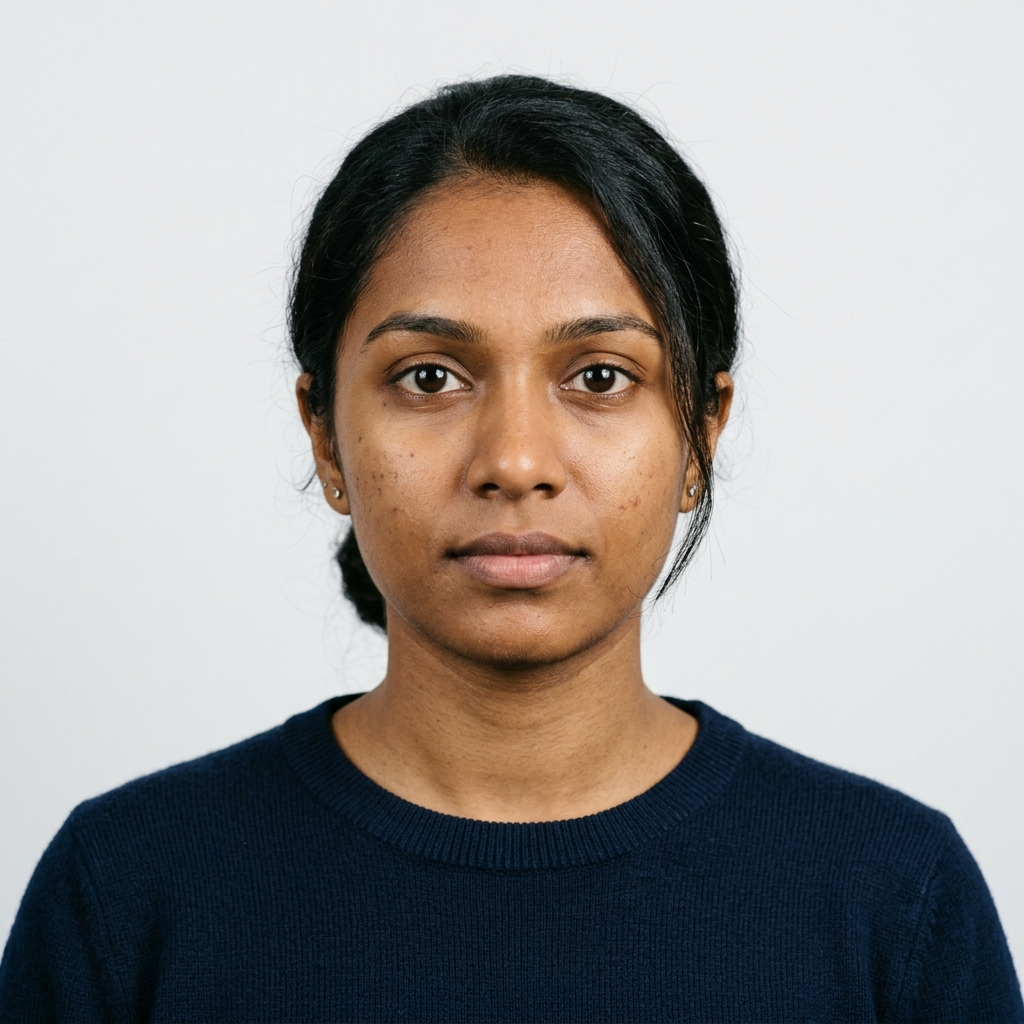
\includegraphics[width=1.7cm,height=1.7cm]{person_profile.jpg}};

  % Profile details on right
  \node[anchor=west, text=ink!70, font=\fontsize{6.5}{8}\selectfont\twfont\bfseries] at (-1.2,3.10) {PROFILE FILE $\cdot$ TARGET \#4091};
  \node[anchor=west, text=ink, font=\dispfont\Large\bfseries] at (-1.2,2.70) {PERSON OF INTEREST};
  \node[anchor=west, text=ink!80!boardbg, font=\fontsize{7}{8.5}\selectfont\twfont] at (-1.2,2.25) {LOCATION: DHAKA, BD \quad AGE: 24};
  \node[anchor=west, text=ink!80!boardbg, font=\fontsize{7}{8.5}\selectfont\twfont] at (-1.2,1.95) {POSTS: 17 \quad STATUS: NORMAL USER};
  \draw[ink!20, line width=0.5pt] (-1.2,1.68) -- (3.6,1.68);

  \node[anchor=center, text=ink!90, font=\fontsize{7.5}{9}\selectfont\twfont\bfseries, align=center]
    at (0,0.95) {IDENTITY RESOLVED THROUGH CONNECTIONS};

  \node[visible on=<2->, bankbadge] (bank2) at ( 0.0, 4.0) {VERIFIED BANK};
  \node[visible on=<2->, scambadge] (sl2)   at (-4.8, 0.0) {FLAGGED SCAM OPERATOR};
  \node[visible on=<2->, scambadge] (sr2)   at ( 4.8, 0.0) {FLAGGED FRAUD RING};
  \draw[gold, line width=1.4pt, visible on=<2->] (0,3.4)     -- (bank2.south);
  \draw[gold, line width=1.4pt, visible on=<2->] (-1.8,0.5)  -- (sl2.north east);
  \draw[gold, line width=1.4pt, visible on=<2->] ( 1.8,0.5)  -- (sr2.north west);

  \node[visible on=<3->, anchor=north, text=gold, font=\fontsize{13}{16}\selectfont\sffamily\bfseries,
        align=center] at (0,-1.0)
    {The Answer Was in the Connections.};
\end{tikzpicture}
\end{frame}

% --- 17.2: Final Close · The Takeaway & Thank You ---
\begin{frame}[plain]
\kicker{SCENE 17 / 17 \quad FINAL CLOSE}
\begin{tikzpicture}[remember picture,overlay,shift={(current page.center)}]
  \node[visible on=<2->, anchor=center, text=gold, font=\dispfont\fontsize{52}{46}\selectfont]
    at (0, 0.0) {Thank you.};

  \node[visible on=<2->, anchor=south, text=dimtext, font=\fontsize{9}{11}\selectfont\twfont, align=center]
    at (0, -2.0) {QUESTIONS \& DISCUSSION};
\end{tikzpicture}
\end{frame}

\end{document}
